\documentclass[11pt,a4paper,oneside,openany]{report}
\usepackage[a4paper,margin=27mm,headheight=15pt]{geometry}
\usepackage[T1]{fontenc}
\usepackage{lmodern}
\usepackage{amsmath,amssymb,amsthm,mathtools}
\usepackage{graphicx,booktabs,longtable,tabularx,array,multirow}
\usepackage[dvipsnames]{xcolor}
\usepackage{microtype}
\usepackage{enumitem}
\usepackage{caption}
\usepackage{float}
\usepackage[round,authoryear]{natbib}
\usepackage{xurl}
\usepackage{fancyhdr}
\usepackage{titlesec}
% Install hyperlink anchors after sectioning changes; cleveref must remain last.
\usepackage[colorlinks=true,linkcolor=MidnightBlue,citecolor=MidnightBlue,urlcolor=MidnightBlue,bookmarksnumbered=true]{hyperref}
\usepackage[capitalize,noabbrev,nameinlink]{cleveref}
\graphicspath{{../figures/}}
\captionsetup{font=small,labelfont=bf,skip=7pt}
\setlength{\parskip}{4pt}
\setlength{\parindent}{1.2em}
\setlength{\emergencystretch}{2em}
\setlist{nosep,leftmargin=*}
\renewcommand{\arraystretch}{1.15}
\titleformat{\chapter}[display]{\normalfont\huge\bfseries\raggedright\hyphenpenalty=10000\exhyphenpenalty=10000}{\chaptertitlename\ \thechapter}{10pt}{\Huge}
\titleformat{\section}{\normalfont\Large\bfseries\raggedright\hyphenpenalty=10000\exhyphenpenalty=10000}{\thesection}{1em}{}
\titleformat{\subsection}{\normalfont\large\bfseries\raggedright\hyphenpenalty=10000\exhyphenpenalty=10000}{\thesubsection}{1em}{}
\titlespacing*{\chapter}{0pt}{-12pt}{24pt}
\pagestyle{fancy}
\fancyhf{}
\fancyhead[L]{\small\nouppercase{\leftmark}}
\fancyfoot[C]{\thepage}
\renewcommand{\headrulewidth}{0.3pt}
\newtheorem{theorem}{Theorem}[chapter]
\newtheorem{proposition}[theorem]{Proposition}
\newtheorem{lemma}[theorem]{Lemma}
\newtheorem{corollary}[theorem]{Corollary}
\theoremstyle{definition}
\newtheorem{assumption}[theorem]{Assumption}
\newtheorem{definition}[theorem]{Definition}
\theoremstyle{remark}
\newtheorem{remark}[theorem]{Remark}
\newcommand{\E}{\mathbb{E}}
\newcommand{\R}{\mathbb{R}}
\newcommand{\Prob}{\mathbb{P}}
\newcommand{\sourcesupp}[1]{\hyperlink{#1}{Source supplement~\texttt{#1}}}
\newcommand{\dif}{\mathop{}\!\mathrm{d}}
\numberwithin{equation}{chapter}

\hypersetup{pdftitle={Stability and identification in inhibitory earthquake models},pdfsubject={Research manuscript}}
\title{Stability and identification in inhibitory earthquake models\\[12pt]\large Restricted mathematics, nuisance sensitivity and predictive evidence}
\author{\small Collaborators: \href{https://github.com/Drefetr}{Drefetr}, \href{https://github.com/magna-nz}{magna-nz};\\[3pt]\small Argon, Astra, Claude, DeepSeek, Sol}
\date{18 October 2026}
\begin{document}
\hypersetup{pageanchor=false}
\maketitle
\begin{abstract}
Event clustering and event-dependent inhibition can coexist in a point process, yet a plausible physical construction does not ensure that their contributions can be distinguished from an observed catalogue. This manuscript studies that distinction for marked earthquake models with relaxation memory. It separates an autonomous physical loading model from a finite-horizon diagnostic with an independently specified background, and distinguishes finite positive exponential mixtures from exact fractional memory.

The mathematical analysis gives restricted first-moment stability and stationary-balance results for finite-mode processes, explains how these can coexist with infinite stationary second moments, and identifies, in no-feedback submodels, explicit obstructions to an unrestricted exact-memory extension. Structural identification at positive inhibition is established only under the stated observation and mark assumptions; at zero inhibition a separately varied stress-memory kernel disappears from the diagnostic observation law. Conditional likelihood identities and positive-inhibition response calculations provide useful finite-history tools without supplying general boundary asymptotics or a universal catalogue-size requirement.

Saved controlled experiments distinguish observation-law separability from the performance of procedures that estimate nuisance structure. A known-law test detected all 150 saved alternatives, with 50 rejections among 1,000 separate null queries. Detection was 123/150 when background level was estimated with trend supplied, and 68/150 when level and trend were both estimated. These are exploratory, procedure-specific calibrated comparisons on reused histories, not a causal decomposition or a guarantee of composite-test performance. In a reconstructed 913-event New Zealand catalogue, the declared shared-inhibition recipe did not improve predictive score over its noninhibited Mittag--Leffler comparator in any of three test periods; most of its aggregate disadvantage occurred in the first period. The results support a bounded mathematical and methodological contribution together with negative predictive evidence about the tested recipes. They establish neither the presence nor the absence of a shared physical stress-memory mechanism.
\end{abstract}

\clearpage
\pagenumbering{roman}
\hypersetup{pageanchor=true}
\tableofcontents
\clearpage
\pagenumbering{arabic}
\chapter{Questions and contribution}
\label{ch:introduction}

An earthquake changes the conditions under which later earthquakes occur. A statistical model may represent some of that change as triggering, which raises the subsequent event rate, and some as depletion, which lowers a stress-controlled contribution to that rate. Relaxation allows the influence of a past event to persist and then decay. These ingredients make a coherent modelling hypothesis, but the observed sequence of event times and magnitudes does not label which mechanism produced each event. A fitted inhibitory term can also compete with a flexible background, an alternative triggering kernel, or an imperfect observation model.

The central question of this manuscript is therefore not simply whether an inhibitory model can be fitted. It is when its event-dependent contribution can be learned, what mathematical assumptions make its dynamics legitimate, and what the available predictive comparisons actually support. The distinction matters in both directions. A weak fitted detector need not mean that two specified generating laws are intrinsically indistinguishable. Conversely, a strong detector supplied with the generating parameters need not show that an unknown-parameter procedure can achieve the same performance. Both questions must be kept separate from identifying a physical mechanism in a real catalogue.

The evidence assembled here supports a restricted, positive mathematical contribution and a qualified negative empirical conclusion. Finite-mode stability, particular identification statements, and finite-history likelihood identities remain useful results under explicit hypotheses. Controlled experiments show substantial changes in calibrated detection when background nuisance structure is estimated. The tested inhibited recipes, however, have not demonstrated improved predictive score on the reconstructed observed catalogue. Neither physical inhibition nor its physical absence follows from that comparison.

The investigation developed from an earlier circulated draft. The current public manuscript is a separate restricted analysis with independently reconstructed computations; it does not reproduce the earlier draft's original calculation. The earlier draft is not redistributed, and its frozen catalogue, original fitting code, complete optimization records and editable source have not been recovered. The public implementation and selected summaries document the present reconstruction, with their availability distinguished in Appendix~\ref{app:evidence}.

\section{From a material hypothesis to an observation law}
\label{sec:intro_material_observation}

A viscoelastic motivation suggests that one relaxation function might describe several responses to an event: the persistence of its stress drop, the accumulated effect of loading, and a triggering density related to the derivative of relaxation. This is a strong modelling restriction. Demonstrating that its components are mathematically compatible is different from showing that the restriction can be distinguished from other explanations using event observations.

The analysis consequently uses two models for different purposes. The physical loading construction retains a latent stress state, a loading history and fresh event marks. Its finite-mode representation permits a Markov description and a scoped stability analysis. The diagnostic model instead specifies a deterministic background independently and asks how identifiable inhibition changes a finite observation law. In abbreviated notation it has intensity
\begin{equation}
 \lambda_\eta(t)=B(t)\exp\{-\eta G_s(t)\}+nH_e(t),
 \qquad \eta\geq 0.
 \label{eq:intro_diagnostic}
\end{equation}
Here $G_s$ is a marked depletion history, $H_e$ is normalized marked triggering, and both use events strictly before $t$. The background $B$ can vary with calendar time. The parameter $\eta$ is a diagnostic inhibition coefficient; it is not automatically the physical stress coefficient of the loading model. The distinction is developed before any theorem or experiment in \cref{ch:models}.

This separation makes the scope of a conclusion visible. An invariant-law theorem for an autonomous finite-mode process does not apply merely because a nonstationary diagnostic uses a similar kernel. A test of inhibition against no inhibition does not by itself test equality of two physical memory functions. A finite-window numerical approximation does not establish a stationary infinite-memory limit. These are different mathematical and observational questions rather than competing descriptions of the same result.

\section{Four questions answered at different levels}
\label{sec:intro_questions}

\begin{enumerate}
 \item \textbf{When is the proposed process well defined and stable?} The finite-mode analysis gives conditions for construction, non-explosion, an invariant law, first moments and convergence in a specified weighted cost. Heavy-tailed marks require attention to the particular moments used. Explicit no-feedback counterexamples show why finite-mode results do not justify an unrestricted exact-memory theorem.
 \item \textbf{What can the observation law identify?} A stress-memory parameter disappears at zero feedback under the stated finite-nuisance or diagnostic conditions. Positive-feedback identification is possible in a restricted full-law experiment with known transforms, empty history and sufficiently rich mark support. Such a statement does not guarantee stable estimation from a finite catalogue.
 \item \textbf{How does estimating nuisance structure change detection?} Controlled comparisons use the same histories, procedure-specific null reference scores and separate null queries. They distinguish strong separation of a fully specified pair from weaker performance when an uninhibited explanation may change its nuisance parameters. The comparison does not identify a unique physical cause or an avoidable fraction of algorithmic loss.
 \item \textbf{Does the additional inhibited structure improve observed prediction?} A chronological comparison evaluates declared recipes using complete predictive scores. The shared-inhibition recipe loses to its noninhibited Mittag--Leffler triggering comparator in each of three test periods, while an Omori comparator scores better than both recipes. Reused periods and different kernel flexibility limit the interpretation to those exploratory recipes.
\end{enumerate}

The first two questions concern dynamics and equality of probability laws. The third concerns a specified testing procedure under a declared generator. The fourth concerns the predictive performance of fitted recipes on an observed catalogue. Evidence at one level can guide another, but cannot replace it.

\section{Relation to existing work}
\label{sec:related_work}

\subsection{Triggering and fractional relaxation}

Self-exciting point processes provide a natural representation of event clustering. Classical work by \citet{Hawkes1971} develops their second-order structure and also illustrates that second-order properties need not uniquely distinguish different process constructions. That observation is relevant to physical interpretation: a recognizable correlation pattern is not, on its own, a unique mechanism assignment.

Mittag--Leffler earthquake triggering is already developed by \citet{DavisBaeumerWang2024}. Their construction uses a fractional relaxation function and a corresponding triggering density, with magnitude-dependent productivity. The triggering component studied here is inherited from that line of work after parameter relabelling; introducing it is not a contribution of this manuscript. The additional target is a restriction linking event-dependent background depletion and triggering memory, together with the mathematical and inferential conditions required to investigate it. The multivariate fractional model of \citet{DavisBaeumerWang2026} further makes mark-category probabilities history dependent. The fresh independent mark assumption used in the present restricted analysis should therefore be read as a modelling boundary, not an advance over history-dependent marks.

\subsection{Excitation correction and spatial structure}

Combining excitation with stress-related correction also predates this work. \citet{PetrilloZhuangLippiello2023} compare statistical mechanisms with catalogues generated by a physical spring-block model and study the interaction of clustering and stress discharge. The relevant distinction lies in the equations: an additive correcting contribution and a positive background multiplied by a relaxing depletion factor need not have the same law or positivity properties. A claim about a shared relaxation restriction must identify that difference explicitly, rather than claim the first combination of excitation and correction.

Spatially heterogeneous backgrounds and different space--time cluster structures are established parts of earthquake point-process modelling \citep{Ogata1998}. The proposed spatial extension in this manuscript is therefore a targeted model-adequacy question. It asks whether localizing depletion adds predictive information beyond matched spatial background and triggering structures. The algebra in \cref{prop:regional_nonclosure} explains why a collection of locally inhibited processes generally cannot be represented by applying a single exponential of pooled depletion to the national background. It does not establish that spatial pooling caused the observed predictive loss.

\subsection{Stability identification and nonregular testing}

General nonlinear Hawkes stability theory \citep{BremaudMassoulie1996} and coupling methods such as those of \citet{HairerMattinglyScheutzow2011} provide an important context for the finite-mode argument. Their hypotheses remain part of the work: a generator drift inequality alone is not a construction, an existence theorem, or a complete contraction proof. The manuscript therefore states the state domain, mark assumptions, coupling cost and finite-mode restrictions alongside the result. It distinguishes a proof within the stated model from a priority claim over all earlier stability theory.

Likewise, the representation and identification results of \citet{DavisKresinBaeumerWang2026} apply under their own linear-model and observation hypotheses. They do not directly settle a nonlinear stress-memory parameter that vanishes from the law at zero feedback. The present restricted identification argument addresses that singularity explicitly, while retaining its dependence on known mark transforms and unbounded mark support.

Testing at such a boundary is not justified by invoking an ordinary likelihood-ratio reference distribution. Work by \citet{Davies1977,Davies1987} identifies the difficulty of a nuisance parameter present only under the alternative. Boundary asymptotics also require regularity conditions of the kind examined by \citet{SelfLiang1987}. These references motivate care; they are not a ready-made calibration theorem for the heavy-tailed inhibited model. For fitted residual diagnostics, \citet{KlingVetter2024} similarly motivates accounting for estimation rather than treating an estimated compensator as known.

\subsection{What remains unresolved about novelty}

The random-excitation spectrum in \citet{BremaudMassoulie2002} is directly relevant to any random-productivity spectral claim. An equation-by-equation comparison of that full result with the earlier manuscript's spectrum has not been completed in the archived audit. This manuscript does not claim a new general Hawkes spectrum on the basis of a missing comparison. Finite-variance formulas also cannot be transferred to a fitted heavy-tail regime without the required moments.

The mathematical contribution is a restricted analysis: a model-specific application of weak Harris theory, fixed-horizon coupling bounds, and self-contained calculations for stationary moments, exact-memory response, observation-law identification and finite-history inference. The approximation discussion corrects the earlier inference from local to half-line Lipschitz continuity. The triggering component is inherited, and the shared depletion/triggering relation is the particular model restriction studied. Appendix~\ref{app:literature_status} classifies the individual results and their primary-source comparisons. No priority claim is made where a full equivalence comparison remains unresolved.

\section{Evidence and interpretation}
\label{sec:intro_evidence}

The observed analysis uses an independently reconstructed GeoNet catalogue. It contains 913 selected events over a 24,394-day window starting in 1960 and ending before 15 October 2026. Although its count matches a count reported in an earlier manuscript, the unavailable historical event list and fitting records have not been recovered. The reconstruction is a new archived snapshot with its own selection rules, not historical reproduction. GeoNet describes its catalogue interfaces as access routes to earthquake parameters \citep{GeoNet2026}; a common provider or matching event count does not make interface snapshots independent catalogues.

The historical controlled studies have a different role. They compare declared laws and procedures, using saved simulated histories and retained failure/recovery policies. When generating nuisance parameters are supplied, the known-law test detects all 150 saved alternatives and rejects 50 of 1,000 separate null queries. Estimating inhibition alone with those nuisance values supplied also detects all 150 alternatives. Estimating background level with trend supplied detects 123, whereas estimating level and trend detects 68. The earlier fuller fitted procedure detects 57 after its own recalibration. These contrasts are substantive evidence about these procedures, with conditional uncertainty and adaptive-reuse qualifications. They are not five independent replications, an additive causal decomposition, or a proof that fixing unknown background values is appropriate for the observed analysis. A subsequent four-procedure continuation is distinguished in Section~\ref{sec:f-continuation} and the accompanying F addendum; its new numerical contract and incomplete null coverage do not replace these historical results.

The predictive comparison contributes a further kind of evidence. The shared-inhibition recipe fails to improve score in each declared test period, with approximately 93.7\% of its total disadvantage in the first. This supports a negative statement about the predictive return from the tested additional structure. It does not supply three independent confirmations against inhibition or identify a geological cause. Event-only spatial group sums and a narrow archived-magnitude substitution help examine particular explanations but do not constitute fitted spatial likelihoods or a complete observation-error analysis.

\begin{table}[tbp]
\centering
\small
\caption{Levels of evidence used in this manuscript. The conclusion in the middle column is intentionally narrower than the excluded inference.}
\label{tab:evidence_levels}
\begin{tabularx}{\textwidth}{@{}>{\raggedright\arraybackslash}p{0.20\textwidth}>{\raggedright\arraybackslash}X>{\raggedright\arraybackslash}X@{}}
\toprule
Evidence & Supported conclusion & Inference not supplied \\
\midrule
Restricted analysis & Results under stated state, kernel and observation assumptions & General nonlinear exact-memory stability or unrestricted physical identification \\
Controlled histories & Calibrated procedure contrasts at the declared generating law & Universal power, avoidable-loss decomposition or real-data nuisance knowledge \\
Chronological scores & Performance ordering of the declared exploratory recipes & Physical exclusion, equal-complexity family ranking or untouched confirmation \\
Source and numerical checks & Specific arithmetic, approximation sensitivity and evidence bindings & Global optimization, catalogue completeness or full historical reproduction \\
\bottomrule
\end{tabularx}
\end{table}

\section{How to read the manuscript}

The exposition follows questions rather than the chronology of research iterations. Chapter~\ref{ch:models} defines the models and their observation conventions. Chapters~\ref{ch:stability} and~\ref{ch:identifiability} develop the mathematical domain and identification boundaries. Chapter~\ref{ch:inference} derives the finite-history likelihood tools and explains what is held fixed in response and testing statements. The remaining main chapters describe the controlled design, report the synthetic and observed evidence, and explain the resulting research decision. A reader primarily interested in the empirical conclusion can read the model definitions, the design and results chapters, and the discussion before returning to the proofs.

The appendices provide an archival source map, numerical/reproducibility boundaries, notation and a focused record of unresolved literature comparisons. Operational recovery histories and file hashes are kept there or in the companion evidence. The main contribution is the connected account of mathematical validity, identification and procedure performance. A bounded locality comparison remains a possible extension of that account.

\chapter{Models, memory and observation}\label{ch:models}

The central difficulty is to separate three objects that are often conflated in stress-release modelling: the physical state that carries memory, the point process that records event occurrence, and the observation model through which events and their marks become data. The finite-mode formulation provides a transparent autonomous physical model. A diagnostic formulation specifies an independent background and separates its suppression from triggering. The distinction matters because stability, approximation and inference make different demands on the model.

\section{The physical finite-mode model}\label{sec:model_physical}

Let \(\vartheta_j>0\) be relaxation rates and let \(w_j>0\), \(\sum_jw_j=1\), be fixed weights. For a constant loading \(\rho\geq0\), write
\[
x_j^*=\frac{\rho}{\vartheta_j},\qquad
\bar x=\sum_jw_jx_j^*,\qquad
\mathcal X=\left\{(Z,U):Z_j\leq x_j^*,\ U_j\geq0\right\}.
\]
The physical stress and excitation reservoir are
\begin{equation}\label{eq:physical-XH}
X=\sum_jw_jZ_j,\qquad H=\sum_jw_jU_j.
\end{equation}
Between events the coordinates relax according to
\begin{equation}\label{eq:finite-flow}
\dot Z_j=\rho-\vartheta_jZ_j,\qquad
\dot U_j=-\vartheta_jU_j.
\end{equation}
The ground event process \(N\) has compensator
\begin{equation}\label{eq:physical-compensator}
\Lambda(t)=\int_0^t\bigl\{\Psi(X(s^-))+H(s^-)\bigr\}\,ds .
\end{equation}
Thus the intensity is evaluated immediately before a possible event and does not include the outcome of that event.

If an event is accepted at time \(T_i\), a fresh mark \(M_i\) is drawn from a fixed law \(F\), conditionally independent of the pre-event history. Only after acceptance does the mark determine the jumps
\begin{equation}\label{eq:finite-jumps}
\Delta Z_j(T_i)=-g(M_i),\qquad
\Delta U_j(T_i)=\vartheta_j\kappa(M_i).
\end{equation}
The functions \(g,\kappa\geq0\) may depend on different aspects of the same mark and may therefore be correlated. Their first moments are denoted by
\[
m_1=\mathbb E_F g(M),\qquad n=\mathbb E_F\kappa(M).
\]
The subcritical condition \(n<1\) will control the expected branching size. Marks affect future event rates, but an accepted event cannot change the probability of its own acceptance.

The stability theorem permits a positive nondecreasing link $\Psi$ that is Lipschitz on the reached upper-bounded stress half-line. One physically signed example is
\begin{equation}\label{eq:physical-link}
\Psi(x)=e^{a+bx},\qquad b\geq0.
\end{equation}
Consequently the loading \(\rho\) acts physically through its effect on the coordinates and hence on \(X\); there is no separate multiplicative loading function in \eqref{eq:physical-compensator}. Model \eqref{eq:finite-flow}--\eqref{eq:physical-link}, with constant \(\rho\) and fixed \(\Psi\), is the autonomous finite-mode model used in the stability and approximation results. See \sourcesupp{S21}.

\section{Memory kernels and exact relaxation}

For the finite-mode flow,
\begin{equation}\label{eq:finite-kernel}
\Phi(t)=\sum_jw_je^{-\vartheta_jt},\qquad
h(t)=-\Phi'(t)=\sum_jw_j\vartheta_je^{-\vartheta_jt}.
\end{equation}
Thus \(\Phi(0)=1\), \(\Phi\) is completely monotone, and \(h\) is a probability density:
\[
\int_0^\infty h(t)\,dt=1-\Phi(\infty)=1.
\]
For arbitrary finite initial coordinates, the coordinate solution gives
\begin{align}
X(t)&=\sum_jw_jZ_j(0)e^{-\vartheta_jt}+\rho\int_0^t\Phi(u)\,du
-\sum_{0<T_i\leq t}g(M_i)\Phi(t-T_i),\label{eq:finite-X-mild}\\
H(t)&=\sum_jw_jU_j(0)e^{-\vartheta_jt}
+\sum_{0<T_i\leq t}\kappa(M_i)h(t-T_i).\label{eq:finite-H-mild}
\end{align}
The first initial term reduces to \(X_0\Phi(t)\) if every stress mode starts at \(Z_j(0)=X_0\); an analogous reduction for excitation requires equal initial excitation coordinates. The current event is excluded when intensity is evaluated at its left limit. General finite initial coordinates need the displayed mode sums.

Formulation \eqref{eq:finite-kernel} is a finite exponential mixture. A non-Markovian relaxation law is obtained by replacing the finite exponential sum with
\begin{equation}\label{eq:mittag-leffler}
\Phi(t)=E_\alpha\!\left(-(t/\tau)^\alpha\right),
\qquad 0<\alpha<1,\quad \tau>0,
\end{equation}
and setting \(h=-\Phi'\). Here \(E_\alpha(z)=\sum_{k=0}^{\infty}z^k/\Gamma(1+\alpha k)\) is the Mittag--Leffler function. For the exact kernel,
\[
\Phi(t)\sim \frac{\tau^\alpha}{\Gamma(1-\alpha)}t^{-\alpha},
\qquad
h(t)\sim \frac{\alpha\tau^\alpha}{\Gamma(1-\alpha)}t^{-1-\alpha}
\]
as \(t\to\infty\). Hence \(h\) is integrable while \(\Phi\) is not. The integrated triggering density is finite, while the integrated stress relaxation of a single release is infinite. The two memory objects therefore have different long-time integrability. The exact kernel is not, for noninteger \(\alpha\), a finite exponential mixture; it therefore carries genuine infinite-dimensional memory.

\begin{figure}[htb]
\centering
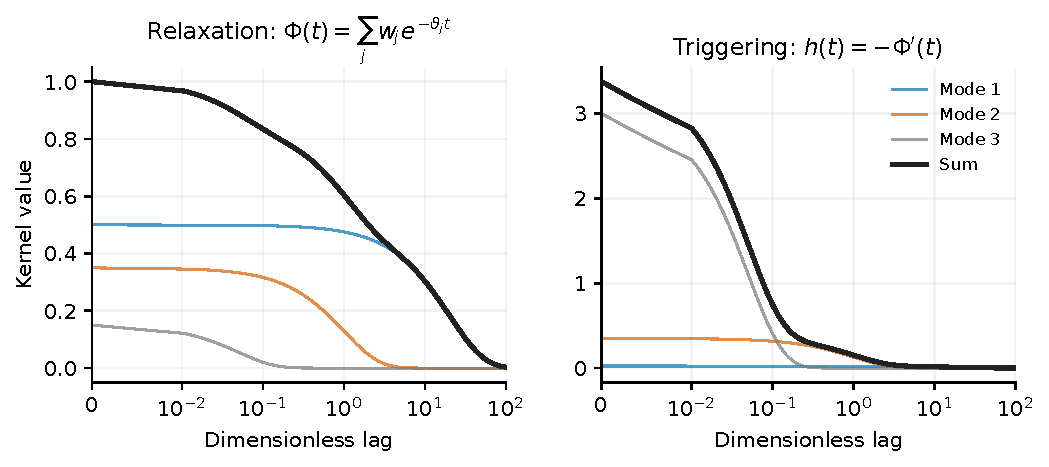
\includegraphics[width=0.95\linewidth]{finite_memory.pdf}
\caption{A dimensionless toy finite mixture with weights $(0.5,0.35,0.15)$ and rates $(0.05,1,20)$. The relaxation $\Phi$ and its negative derivative $h$ weight the same modes differently. Curves are direct evaluations of the displayed finite sums; they are not fits, simulations or an exact Mittag--Leffler kernel.}
\label{fig:finite_memory}
\end{figure}

In the physical model \(w_j\) is dimensionless, \(\vartheta_j\) and \(h\) have inverse-time units, \(\Phi\) is dimensionless, \(\rho\) is stress per unit time, and \(g(M)\) is measured in stress units. The jump \(\vartheta_j\kappa(M)\) has the units of \(U_j\). With no history, the sums in \eqref{eq:finite-X-mild}--\eqref{eq:finite-H-mild} are empty.

\section{The diagnostic model and observation}\label{sec:model_diagnostic}

For diagnostic work, retain a stress relaxation kernel \(\Phi_s\) and a normalized triggering density \(h_e\), initially allowing them to vary separately. Let \((T_i,Q_i)\) denote the accepted event times and their marks. Define the strictly prior cumulative release and excitation sums by
\begin{equation}\label{eq:diagnostic-sums}
G_s(t)=\sum_{0<T_i<t}g(Q_i)\Phi_s(t-T_i),
\qquad
H_e(t)=\sum_{0<T_i<t}\kappa(Q_i)h_e(t-T_i),
\end{equation}
and adopt the diagnostic intensity
\begin{equation}\label{eq:diagnostic-intensity}
\lambda_\eta(t)=B(t)\exp\{-\eta G_s(t)\}+nH_e(t).
\end{equation}

\begin{figure}[htb]
\centering
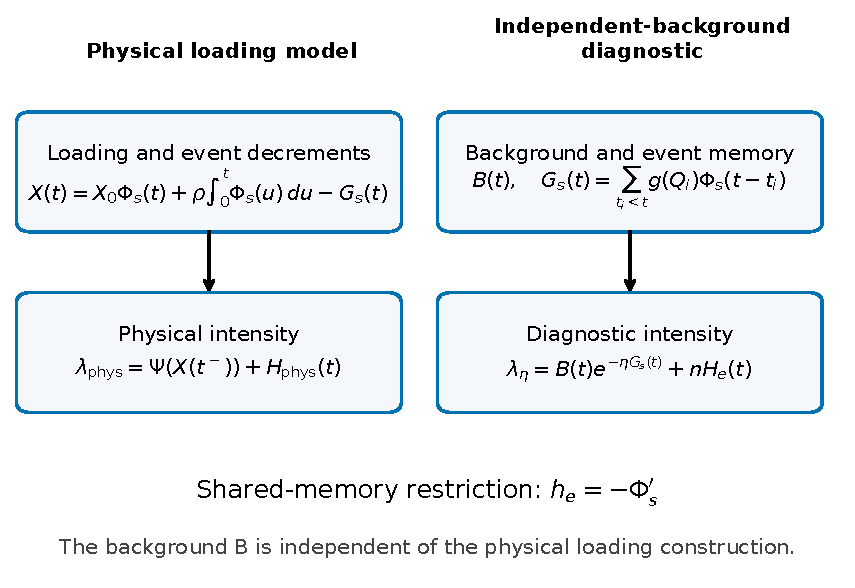
\includegraphics[width=0.95\linewidth]{model_architecture.pdf}
\caption{Physical loading and the independent-background diagnostic answer different questions. The physical model feeds loading through stress; the diagnostic specifies a background and suppresses its contribution by accumulated release. Triggering remains additive. The unit-productivity convention, with $n$ outside $H_e$, applies to the diagnostic.}
\label{fig:model_architecture}
\end{figure}
The baseline \(B(t)\) is deterministic at fixed parameters and specified independently of the stress-kernel family. A useful choice is \(B(t)=\exp\{a+d(2t/T-1)\}\). It is not generated by stress loading or by the marks. The strict inequalities in \eqref{eq:diagnostic-sums} are deliberate: an event is accepted before its mark is drawn, so its own release and productivity cannot enter its intensity.

This section adopts a convention change once and for all: diagnostic productivity is scaled to have unit mean,
\[
\mathbb E_F\kappa(Q)=1,
\]
while the coefficient \(n\) is retained \emph{outside} \(H_e\) in \eqref{eq:diagnostic-intensity}. In the physical model, by contrast, \(n=\mathbb E_F\kappa(M)<1\) is the mean carried by the productivity marks themselves. The diagnostic normalisation removes that mean from the marks and displays it explicitly as a coefficient. This is a bookkeeping convention, not an assertion that realised productivity is one, and it is not used to reinterpret the autonomous physical stability theorem.

The physical exponential link \eqref{eq:physical-link} embeds loading through \(X\): a constant \(\rho\) shifts the physical stress state and therefore changes \(\Psi(X)\). The time-dependent baseline \(B(t)\) in \eqref{eq:diagnostic-intensity} is an independently specified background. It does not replace \(\Psi(X)\) in the autonomous invariant-law theorem; that theorem does not cover externally varying \(B(t)\).

The shared subfamily imposes the identity \(h_e=-\Phi_s'\). This has substantive model content: the instantaneous excitation density is the negative derivative of the same kernel that governs stress relaxation. Consequently the decay of past stress and the contribution of a mark to the future compensator come from one memory structure, including its normalisation. Choices of \(\Phi_s\) and \(h_e\) that do not satisfy this identity define a separate-memory model. Normalization alone does not impose their equality. See \sourcesupp{S22}.

A ground process records only the event times \(T_i\), whereas a marked process records the pairs \((T_i,Q_i)\). The ground law is a projection of the marked law. The event-time contribution to a joint marked likelihood, evaluated using observed past marks, is a different object from the marginal likelihood of times alone. Event times alone generally do not identify \(g\) and \(\kappa\) separately, nor their within-mark dependence, without an additional mark model. Conversely, the marked likelihood includes both ground acceptance probabilities and mark densities. Since marks are fresh after acceptance, past marks enter \eqref{eq:diagnostic-intensity} through the strict sums \eqref{eq:diagnostic-sums}, while a newly drawn mark first affects the future. This observational distinction is essential: marginalizing to times alone and evaluating a joint marked likelihood answer different questions.



The likelihoods studied below condition on a declared starting history. Empty prehistory is a model assumption rather than a statement that no earlier earthquakes occurred. Likewise, a fresh common mark law does not establish completeness or homogeneous measurement of the observed catalogue. Unobserved parents, omitted regions and uncertain magnitudes can change the relationship between the mathematical history and its recorded counterpart. The subsequent identification statements concern the declared complete marked process; their transfer to an earthquake catalogue requires an observation model.

\chapter{Stability, approximation and exact memory}\label{ch:stability}

The finite-mode model admits a comparatively complete stability theory under autonomous loading and integrable marks. The theory combines a branching domination, a Lyapunov function, a synchronous coupling and a small-set estimate. Kernel approximation is then controlled on a fixed horizon. Finally, exact memory reveals a sharp obstruction without feedback and a resolvent response for an associated linear system; neither statement supplies a general nonlinear stationary theory.

\begin{figure}[htb]
\centering
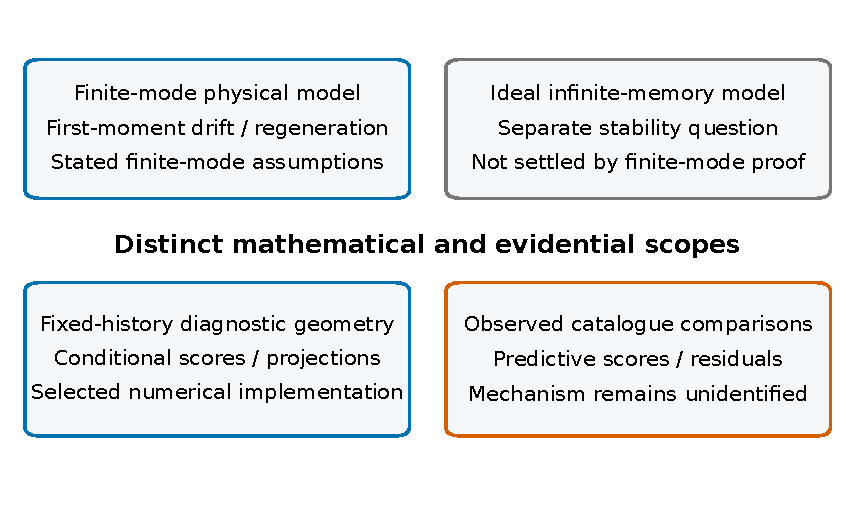
\includegraphics[width=0.95\linewidth]{theory_scope.pdf}
\caption{The positive results have different assumption sets and limiting regimes. Finite-mode invariant laws, fixed-horizon approximation and the auxiliary response do not combine into a nonlinear exact-memory ergodicity theorem.}
\label{fig:theory_scope}
\end{figure}

\section{Autonomous finite-mode stability}\label{sec:finite-stability}

Return to the physical convention \(n=\E _F\kappa(M)\). Suppose \(m_1<\infty\), \(n<1\), and \(\Psi:(-\infty,\bar x]\to(0,\infty)\) is nondecreasing and Lipschitz on the whole half-line. Write \(\bar\Psi=\Psi(\bar x)\). Put
\[
y_j=x_j^*-Z_j,\qquad Y=\sum_jw_jy_j,\qquad
W=\sum_j\frac{w_jU_j}{\vartheta_j},\qquad V=1+Y+cW,
\]
where
\begin{equation}\label{eq:c-choice}
c>\frac{m_1}{1-n}.
\end{equation}
The following theorem concerns constant \(\rho\) and fixed \(\Psi\); it is not a theorem about a time-varying diagnostic baseline.

\begin{theorem}[Finite-mode stability]\label{thm:finite_mode}
From every finite state in \(\mathcal X\), the autonomous finite-mode model has a pathwise unique, non-explosive, cadlag strong Markov construction and a Feller semigroup \(P_t\). There is a unique invariant probability \(\pi\) satisfying \(\pi(V)<\infty\). For suitable positive \(\epsilon,\beta,C,r\), with
\[
\|z-z'\|=\sum_jw_j\bigl(|Z_j-Z'_j|+|U_j-U'_j|\bigr),\qquad
d_\epsilon(z,z')=1\wedge\frac{\|z-z'\|}{\epsilon},
\]
and
\[
\widetilde d(z,z')=
\sqrt{d_\epsilon(z,z')\{1+\beta V(z)+\beta V(z')\}},
\]
one has
\begin{equation}\label{eq:weighted-contraction}
W_{\widetilde d}(P_t(z,\cdot),\pi)
\leq Ce^{-rt}\sqrt{1+V(z)},\qquad t\geq0.
\end{equation}
In particular, \(P_t(z,\cdot)\) converges weakly to \(\pi\).
\end{theorem}

Here \(W_c\) is the infimum of the expected cost \(c\) over couplings. The weighted cost \(\widetilde d\) need not satisfy a triangle inequality; the conclusion is not a total-variation mixing statement.

The constants generally depend on the rates, weights, \(m_1\), \(n\), the Lipschitz constant of \(\Psi\) and \(\bar\Psi\). No uniformity is claimed as \(\vartheta_{\min}=\min_j\vartheta_j\) tends to zero; the contractive time and the selected radius may deteriorate in that limit.

\begin{proof}
\emph{Construction and nonexplosion.} Use a marked Poisson embedding with thinning by the predictable intensity \(\Psi(X)+H\). The process is dominated by a marked Hawkes process with immigration \(\bar\Psi\), kernel
\[
h_d(t)=\sum_jw_j\vartheta_je^{-\vartheta_jt},
\]
and initial excitation \(\sum_jw_jU_j(0)e^{-\vartheta_jt}\). The latter integrates to \(W(z)\), and each cluster has expected total size \(1/(1-n)\). For every nonnegative mark weight \(\omega\) with finite mean,
\begin{equation}\label{eq:cluster-moment}
\E _z\sum_{T_i\leq T}\omega(M_i)
\leq\frac{\E _F\omega(M)}{1-n}
\{\bar\Psi T+W(z)\}.
\end{equation}
A generation is created before its marks are drawn, so \eqref{eq:cluster-moment} remains valid when \(\omega\) and \(\kappa\) are correlated. Finite expected counts imply nonexplosion; the deterministic flow and fresh Poisson increments yield the strong Markov property.

\emph{Lyapunov estimate.} Since the flow gives \(\dot Y=-\sum_jw_j\vartheta_jy_j\) and \(\dot W=-H\), while a jump adds \((g,\kappa)\), the extended generator satisfies
\[
\mathcal AV
=-\sum_jw_j\vartheta_jy_j-\delta H+(m_1+cn)\Psi(X),
\qquad
\delta=c(1-n)-m_1>0.
\]
Because \(\Psi(X)\leq\bar\Psi\) on \(\mathcal X\), direct comparison with the positive relaxation terms gives
\begin{equation}\label{eq:generator-bound}
\mathcal AV\leq-\omega V+D,
\end{equation}
where
\[
K_0=(m_1+cn)\bar\Psi,\qquad
\omega=\vartheta_{\min}\min\{1,\delta/c\},\qquad
D=\omega+K_0.
\]
The weighted jump bound \eqref{eq:cluster-moment} makes the stopped compensated jump integral integrable. Applying the product formula to \(e^{\omega t}V(z_t)\) and then Fatou's lemma gives
\begin{equation}\label{eq:lyap-moment}
P_tV(z)\leq e^{-\omega t}V(z)+\frac{D}{\omega}(1-e^{-\omega t}).
\end{equation}

\emph{Coupling and smallness.} Couple two copies synchronously until their first unmatched event \(\sigma\). Identical jumps cancel before \(\sigma\), so
\[
\|z_t-z'_t\|\leq e^{-\vartheta_{\min}t}\|z-z'\|
\]
on \(\{\sigma>t\}\). Bounding the compensator of the difference of their rates by \(L\|z_t-z'_t\|\), with \(L=\max\{L_\Psi,1\}\), gives
\[
\mathbb P(\sigma\leq t)\leq
\frac{L}{\vartheta_{\min}}\|z-z'\|.
\]
Thus, whenever \(d_\epsilon(z,z')<1\),
\begin{equation}\label{eq:coupling-contraction}
W_{d_\epsilon}(P_tz,P_tz')
\leq\left(e^{-\vartheta_{\min}t}
+\frac{L\epsilon}{\vartheta_{\min}}\right)d_\epsilon(z,z').
\end{equation}
Choose \(\epsilon\) small and then \(t\) large enough to make the coefficient less than one up to the prescribed margin. Sublevel sets \(\{V\leq R\}\) are compact and have finite diameter \(D_R\). On such a set, event-free flow decreases both \(Y\) and \(W\), and the event rate is at most \(\Lambda_R=\bar\Psi+\vartheta_{\max}R/c\). 
Use the same marked Poisson random measure $\Pi$ for both
copies, with intensity $\dif s\,\dif u\,F(\dif m)$ and the
usual acceptance threshold. The event
\[
 \Pi\bigl([0,t]\times[0,\Lambda_R]\times\mathsf M\bigr)=0
\]
has probability $e^{-\Lambda_Rt}$, since $F$ has total mass one. On this
event both copies follow their event-free flows and their rates remain at
most $\Lambda_R$, so neither jumps. Thus the synchronous coupling gives probability at least $e^{-\Lambda_Rt}$ that neither copy jumps. Once \(e^{-\vartheta_{\min}t}D_R\leq\epsilon/2\),
\[
\sup_{V(z),V(z')\leq R}W_{d_\epsilon}(P_tz,P_tz')
\leq1-\tfrac12e^{-\Lambda_Rt}<1.
\]
The same coupling shows that the state at a fixed time converges in probability as the initial state varies continuously. Expectations of bounded continuous functions therefore converge, establishing the Feller property. To choose a common time for contraction and smallness, first fix \(R=4D/\omega\) from the Lyapunov bound, then choose time sufficiently large for both inequalities.

Together with \eqref{eq:lyap-moment} this verifies the Lyapunov, contraction and smallness hypotheses of \citet{HairerMattinglyScheutzow2011}, Theorem~4.8 in the author-final version. Their Corollary~4.11 adds existence under the Feller and completeness conditions used here. Existence also follows from tight time-averaged laws, compact sublevels and \eqref{eq:lyap-moment}. The contraction time provided by the theorem may be later than the time used to check the hypotheses. Replacing \(d_\epsilon\) by \(\widetilde d\) and iterating the resulting contraction, while using \eqref{eq:lyap-moment} for the residual time, gives \eqref{eq:weighted-contraction}. No second mark moment is required.

To see that every invariant probability has the same finite moment without subtracting potentially infinite integrals, suppose \(PV\leq aV+b\) with \(a<1\), and put \(f_K(v)=\min(v,K)\). If \(\nu\) is invariant, concavity gives
\[
\nu\{f_K(V)-f_K(aV+b)\}\leq0.
\]
For \(K\geq b/(1-a)\), the integrand is at least
\([(1-a)V-b]\mathbf 1_{\{V\leq K\}}\). Hence
\(\nu(V\mathbf 1_{\{V\leq K\}})\leq b/(1-a)\). Monotone convergence and \eqref{eq:lyap-moment} yield \(\nu(V)\leq D/\omega\). The weak Harris theorem supplies uniqueness.
\end{proof}

Under the invariant law, let \(\Lambda=\pi(\Psi(X)+H)>0\). Stationarity in the coordinate equations, justified by the weighted jump bound, gives
\[
\pi(U_j)=n\Lambda,\qquad
\pi(Z_j)=\frac{\rho-m_1\Lambda}{\vartheta_j},\qquad
\Lambda=\frac{\pi(\Psi(X))}{1-n},
\]
and hence
\[
\pi(X)=(\rho-m_1\Lambda)\sum_j\frac{w_j}{\vartheta_j}.
\]
Under \(\mathbb P_\pi\), intensity ergodicity and the compensated counting martingale give \(N(t)/t\to\Lambda\), while the fresh-mark strong law gives \(t^{-1}\sum_{T_i\leq t}g(M_i)\to m_1\Lambda\).

\begin{proposition}[Infinite stationary second moments]\label{prop:heavy-moments}
If \(\E _Fg(M)^2=\infty\), then \(\pi(Y^2)=\infty\) and consequently \(\pi(X^2)=\infty\). If \(\E _F\kappa(M)^2=\infty\), then \(\pi(W^2)=\infty\) and consequently \(\pi(H^2)=\infty\).
\end{proposition}

\begin{proof}
Let \(\Phi_d(t)=\sum_jw_je^{-\vartheta_jt}>0\). The mild equations for the nonnegative depletion modes \(y_j\) and the integrated excitation modes give, on any stationary interval of length \(t\),
\[
Y(0)^2\geq\Phi_d(t)^2\sum_{-t<T_i\leq0}g(M_i)^2,
\qquad
W(0)^2\geq\Phi_d(t)^2\sum_{-t<T_i\leq0}\kappa(M_i)^2.
\]
Replace a squared mark by \(g_K^2=(g\wedge K)^2\). Fresh-mark compensation, applied before each mark is revealed, gives
\[
\E _\pi\sum_{-t<T_i\leq0}g_K(M_i)^2
=\E _Fg_K(M)^2\int_{-t}^0\E _\pi\lambda_s\,\dif s
=t\Lambda\E _Fg_K(M)^2.
\]
Thus
\(\pi(Y^2)\geq\Phi_d(t)^2t\Lambda\E _Fg_K(M)^2\).
Letting \(K\uparrow\infty\) proves the first implication. The productivity argument is identical. Since \(X=\bar x-Y\), infinite \(\pi(Y^2)\) implies infinite \(\pi(X^2)\). Since \(W\) and \(H\) are comparable through the finitely many positive rates, infinite \(\pi(W^2)\) implies infinite \(\pi(H^2)\).
\end{proof}

The argument concerns the corresponding jump transform: it asserts stress divergence when the stress-mark second moment diverges, and excitation divergence when the productivity second moment diverges. Finite first-moment stability and infinite stationary variance coexist. A quadratic theorem under stronger finite-moment assumptions is not contradicted; those stronger assumptions cannot be inferred for an untruncated heavy-tailed fitted law.

\section{Fixed-horizon kernel approximation}

Let \(\Phi\) and \(\Phi_d\) be nonnegative decreasing absolutely continuous kernels, normalised to one at zero and tending to zero at infinity, so that \(h=-\Phi'\) and \(h_d=-\Phi_d'\) are probability densities. Use the same finite initial stress and constant loading, no prehistory, fresh marks, and the first-moment assumptions above. Let \(\Psi\) be positive, nondecreasing and locally Lipschitz on \(\mathbb R\). For fixed \(T<\infty\), put
\[
B=A_T=|X_0|+\rho T,\qquad
K_T=\frac{\Psi(B)T}{1-n},
\]
\[
\Delta_\Phi=\sup_{[0,T]}|\Phi_d-\Phi|,
\qquad
\Delta_h=\int_0^T|h_d-h|.
\]

\begin{proposition}[Quantitative half-line approximation]\label{prop:quantitative-kernel}
If \(\Psi\) is Lipschitz on \((-\infty,B]\) with constant \(L_B\), then, under the same Poisson-measure coupling,
\begin{equation}\label{eq:quantitative-kernel}
\mathbb P(\text{marked catalogues differ on }[0,T])
\leq\min\{1,\;L_BT(A_T+m_1K_T)\Delta_\Phi+nK_T\Delta_h\}.
\end{equation}
For \(\Psi(x)=e^{a+bx}\), \(b\geq0\), one may take \(L_B=be^{a+bB}\).
\end{proposition}

\begin{proof}
All stresses remain at most \(B\). Until the two coupled processes first separate,
\[
|X_d(s)-X(s)|
\leq\Delta_\Phi\left(A_T+\sum_{T_i<s}g(M_i)\right),
\]
and the integrated excitation discrepancy is bounded by
\(\Delta_h\sum_{T_i\leq T}\kappa(M_i)\). Common pre-separation events form a subset of the reference events, which are dominated by the Hawkes process with immigration \(\Psi(B)\). Its expected event count is at most \(K_T\), while the corresponding weighted expectations are at most \(m_1K_T\) and \(nK_T\). Bounding the compensated difference of the two event intensities by the stress discrepancy and the excitation discrepancy and integrating its expectation gives \eqref{eq:quantitative-kernel}.
\end{proof}

Local Lipschitz continuity does not support the same linear error bound. It nevertheless gives qualitative convergence through a separate truncation.

\begin{proposition}[Qualitative local approximation]\label{prop:qualitative-kernel}
For \(R>0\), let \(L_R\) be a Lipschitz constant of \(\Psi\) on \([-|X_0|-R,B]\). Then
\begin{equation}\label{eq:qualitative-kernel}
\mathbb P(\text{catalogues differ on }[0,T])
\leq\min\left\{1,\frac{m_1K_T}{R}
+L_RT(A_T+R)\Delta_\Phi+nK_T\Delta_h\right\}.
\end{equation}
\end{proposition}

\begin{proof}
On common prehistories whose cumulative release is at most \(R\), both stresses lie in the compact interval on which \(L_R\) is valid, and the half-line calculation applies with \(R\) in place of the full released mass. The complement has probability at most \(m_1K_T/R\) by Markov's inequality. Fix \(R\), let the two kernel errors tend to zero, and then let \(R\to\infty\).
\end{proof}

Thus half-line Lipschitz continuity gives a quantitative error rate, whereas local Lipschitz continuity gives only qualitative fixed-horizon convergence. A finite half-line constant cannot be inferred from local Lipschitz continuity. Nor do these results exchange the kernel-approximation and long-time limits.

\section{Exact-memory obstruction and response}

Exact memory neither prevents all stationary constructions nor yields a general nonlinear stationary theorem. The first point is visible already in a zero-history model without feedback.

\begin{proposition}[No-feedback obstruction]\label{prop:exact-obstruction}
Let \(0<\alpha<1\), \(\tau>0\), and
\(\Phi(t)=E_\alpha(-(t/\tau)^\alpha)\). Consider the zero-history model with \(X_0=0\), constant immigration rate \(\mu>0\), no triggering, and loading \(\rho=\mu\E  S\). Let \(N(\dif v,\dif S)\) be Poisson with intensity \(\mu\,\dif v\,F_S(\dif S)\), let \(\widetilde N\) be its compensated measure, and define
\[
X(t)=-\int_0^t\Phi(t-v)S\,\widetilde N(\dif v,\dif S).
\]
If \(S=1\), no sequence \(t_k\to\infty\) has a tight subsequence of stress laws for \(\alpha\leq1/2\). If \(P(S>s)=s^{-q}\) for \(s\geq1\) and \(1<q<2\), the corresponding obstruction occurs when \(\alpha q\leq1\). For \(S=1\), \(\alpha>1/2\) admits a stationary two-sided compensated moving average in \(L^2\), and the zero-history one-time laws converge. For Pareto marks, \(\alpha q>1\) admits such a construction in \(L^p\) for every \(1/\alpha<p<q\).
\end{proposition}

\begin{proof}
The finite-interval Poisson exponential formula gives
\begin{equation}\label{eq:obstruction-cf}
\left|\E  e^{iuX(t)}\right|
=\exp\left\{-\mu\int_0^t
\E _F\{1-\cos(uS\Phi(v))\}\,\dif v\right\}.
\end{equation}
For unit marks, the integrand is asymptotic to \(u^2\Phi(v)^2/2\) for fixed \(u\neq0\). For Pareto marks and \(0<x\leq1\), restricting \(S\) to \([1/x,2/x]\) yields
\[
\E _F\{1-\cos(xS)\}
\geq(1-\cos1)(1-2^{-q})x^q.
\]
Since
\(\Phi(v)\sim\tau^\alpha v^{-\alpha}/\Gamma(1-\alpha)\),
the modulus \eqref{eq:obstruction-cf} tends to zero at every nonzero frequency in the stated regimes. Tightness would give a weak subsequential limit; by the continuity theorem its characteristic function would be continuous at zero, but the limit would equal zero at every \(u\neq0\) and one at \(u=0\), a contradiction.

Above the threshold, the two-sided compensated integrals converge in \(L^2\) by the isometry for unit marks. For Pareto marks, choose \(1/\alpha<p<q\). Then \(\E  S^p<\infty\) and \(\int_0^\infty\Phi(v)^p\,\dif v<\infty\), so the compensated Poisson \(L^p\) estimate gives the two-sided construction.
\end{proof}

This is a no-feedback statement. It does not assert nonstationarity of the stress-sensitive nonlinear model, and a stationary compensated construction is not the subtraction of two separately divergent, uncompensated past integrals.

For an auxiliary excitation-inclusive system, a positive stress-to-rate slope changes the response through an integrable resolvent with a heavy tail. Let \(m_1>0\), \(0\leq n<1\) and \(\ell>0\), and consider
\begin{equation}\label{eq:aux-response-equations}
x=-m_1\Phi*y,\qquad
y=\ell x+nh*y+\xi,\qquad
h=-\Phi',
\end{equation}
with zero initial perturbation and additive event-flux forcing \(\xi\). Set
\[
\gamma=m_1\ell,\qquad \beta_{\mathrm{rel}}=1-\alpha,\qquad
a_{\mathrm{rel}}=(1-n)\tau^{-\alpha}.
\]

\begin{proposition}[Excitation-inclusive response]\label{prop:auxiliary-response}
The causal solution of \eqref{eq:aux-response-equations} is
\(x=-m_1R_\gamma*\xi\), where
\begin{equation}\label{eq:response-transform}
\widehat R_\gamma(s)=\frac{1}{s+a_{\mathrm{rel}} s^{\beta_{\mathrm{rel}}}+\gamma}.
\end{equation}
For \(\gamma>0\), \(R_\gamma\) is completely monotone, \(R_\gamma(0+)=1\), \(\int_0^\infty R_\gamma(t)\,\dif t=1/\gamma\), and
\begin{equation}\label{eq:response-tail}
R_\gamma(t)\sim
\frac{a_{\mathrm{rel}}\beta_{\mathrm{rel}}}{\gamma^2\Gamma(1-\beta_{\mathrm{rel}})}t^{-1-\beta_{\mathrm{rel}}}.
\end{equation}
In particular, \(\int_0^\infty tR_\gamma(t)\,\dif t=\infty\).
\end{proposition}

\begin{proof}
Eliminating \(y\) in the Laplace domain gives
\[
\widehat\Phi(s)=\frac{s^{\alpha-1}}{s^\alpha+\tau^{-\alpha}},
\qquad
\widehat h(s)=\frac{\tau^{-\alpha}}{s^\alpha+\tau^{-\alpha}}.
\]
Substitution into \eqref{eq:aux-response-equations} yields
\[
\widehat x(s)=-\frac{m_1s^{\alpha-1}\widehat\xi(s)}
{s^\alpha+\gamma s^{\alpha-1}+(1-n)\tau^{-\alpha}}
=-m_1\widehat R_\gamma(s)\widehat\xi(s),
\]
which is \eqref{eq:response-transform}. The reciprocal of the nonnegative complete Bernstein function \(s+a_{\mathrm{rel}} s^{\beta_{\mathrm{rel}}}+\gamma\) is a Stieltjes function, hence \(R_\gamma\) is completely monotone
\citep[Section~2.1]{MeerschaertToaldo2019}. Its spectral density is
\[
k_\gamma(r)=
\frac{a_{\mathrm{rel}}\sin(\pi\beta_{\mathrm{rel}})r^{\beta_{\mathrm{rel}}}}
{\pi\{[\gamma-r+a_{\mathrm{rel}} r^{\beta_{\mathrm{rel}}}\cos(\pi\beta_{\mathrm{rel}})]^2+
a_{\mathrm{rel}}^2r^{2\beta_{\mathrm{rel}}}\sin^2(\pi\beta_{\mathrm{rel}})\}},
\]
so \(R_\gamma(t)=\int_0^\infty e^{-rt}k_\gamma(r)\,\dif r\). The limits of \eqref{eq:response-transform} at infinity and zero give \(R_\gamma(0+)=1\) and \(\int R_\gamma=1/\gamma\). Near \(r=0\),
\[
k_\gamma(r)\sim
\frac{a_{\mathrm{rel}}\sin(\pi\beta_{\mathrm{rel}})}{\pi\gamma^2}r^{\beta_{\mathrm{rel}}}.
\]
Rescaling the spectral integral and using the gamma reflection formula gives \eqref{eq:response-tail}. The tail exponent \(-1-\beta_{\mathrm{rel}}\) lies between \(-2\) and \(-1\), so the first temporal moment diverges.
\end{proof}

The weak-feedback crossover is equally explicit. Put \(t_\gamma=(a_{\mathrm{rel}}/\gamma)^{1/\beta_{\mathrm{rel}}}\). As \(\gamma\downarrow0\), the probability densities \(\gamma t_\gamma R_\gamma(t_\gamma u)\) on \((0,\infty)\) converge weakly to the law with Laplace transform \((1+z^{\beta_{\mathrm{rel}}})^{-1}\), because
\[
\int_0^\infty e^{-zu}\gamma t_\gamma R_\gamma(t_\gamma u)\,\dif u
=\frac{1}{1+z^{\beta_{\mathrm{rel}}}+z/(\gamma t_\gamma)}
\longrightarrow\frac{1}{1+z^{\beta_{\mathrm{rel}}}}.
\]
At \(\gamma=0\), \(R_0(t)=E_\alpha(-a_{\mathrm{rel}}t^\alpha)\) is not integrable. The crossover is separated from the early-time scale \(a_{\mathrm{rel}}^{-1/\alpha}\) only when \(\gamma\ll a_{\mathrm{rel}}^{1/\alpha}\). This is a statement about an auxiliary impulse response, not a nonlinear mixing time.

A restricted nonlinear observation follows from the same resolvent. For
\[
y=\psi(x)+nh*y+\xi,\qquad \psi(0)=0,
\]
write \(\mathcal E(x)=m_1\psi(x)-\gamma x\). If \(\mathcal E\) is globally Lipschitz with constant \(L<\gamma\), the equivalent map
\[
x=-R_\gamma*(m_1\xi+\mathcal E(x))
\]
is a contraction on bounded causal functions, and
\(\|x\|_\infty\leq m_1\|\xi\|_\infty/(\gamma-L)\). This is only an externally forced auxiliary Volterra result. The positive exponential rate does not satisfy such a global sector condition, since its derivative tends to zero as stress tends to negative infinity. For jointly measurable stationary forcing with an almost surely uniform deterministic bound, the integrable-resolvent fixed-point equation has a unique bounded causal stationary solution by contraction and shift-equivariant Picard iteration, but it does not assert absolute convergence of the two-sided convolution \(\Phi*y\), because \(\Phi\) is not integrable.

The obstruction and resolvent calculation therefore delimit the demonstrated scope. Neither supplies a generic stationary theorem for the nonlinear stress-sensitive exact-memory process.

\subsection{What the auxiliary response omits}

The actual marked process has two noise sources rather than a single prescribed event-flux input. In the physical productivity convention, define compensated marked measures by
\[
\dif M_g=\dif N_g-m_1\lambda\,\dif t,\qquad
\dif M_\kappa=\dif N_\kappa-n\lambda\,\dif t,
\]
where $N_g$ and $N_\kappa$ accumulate the corresponding marks. These martingales are generally correlated: both jump at the same events, and the two transforms of a fresh mark need not be independent. 

\begin{samepage}
Set $Q_\gamma=R_\gamma-nR_\gamma*h$, and let $X^+(t)$ denote post-event stress, including releases at time $t$. For scalar initial stress \(X_0\Phi(t)\), zero initial excitation and no additional prehistory, finite-horizon compensation and the same Laplace-resolvent algebra give the exact identity
\begin{align}
X^+(t)={}&X_0Q_\gamma(t)+\rho\int_0^tQ_\gamma(u)\,\dif u \notag\\
&+[R_\gamma*(\gamma X^+-m_1\Psi(X^+_-))](t) \notag\\
&-\int_{(0,t]}Q_\gamma(t-u)\,\dif M_g(u) \notag\\
&-m_1\int_{(0,t]}(R_\gamma*h)(t-u)\,\dif M_\kappa(u).
\label{eq:marked-resolvent}
\end{align}
\end{samepage}
Here $X^+_-(u)=X^+(u^-)$, and all assertions are on finite horizons under compensator integrability. At an event time, the intensity uses the left limit; the displayed post-event identity must be left-limited consistently if it is used to evaluate that intensity. The deterministic kernels in the two noise terms are bounded and integrable, but this does not by itself control the nonlinear residual in the second line. In particular, the stress can leave any band on which a positive lower slope is available. Establishing tightness or a uniform occupation bound outside that band remains a separate task. The identity explains the relevance of the auxiliary response while retaining the nonlinear term and both correlated mark martingales.

\paragraph{Compensation and cancellation.}
An event-free path has $\dif N_g=\dif N_\kappa=0$, but not
$\dif M_g=\dif M_\kappa=0$. Instead,
\[
  \dif M_g=-m_1\lambda\,\dif t,
  \qquad
  \dif M_\kappa=-n\lambda\,\dif t.
\]
The compensated integrals must therefore be retained even when no event
occurs. The causal kernels satisfy
\[
 Q_\gamma+nR_\gamma*h=R_\gamma,
 \qquad
 Q_\gamma+\gamma R_\gamma*\Phi=\Phi.
\]
For the stated initialization, put
$f=X_0\Phi+\rho(1*\Phi)$, where $(1*\Phi)(t)=\int_0^t\Phi(u)\,\dif u$.
In the following ordinary time convolutions write $X$ for $X^+$, retaining
$X_-$ in the predictable intensity. The original equations give
\[
 X=f-\Phi*\dif N_g,
 \qquad \lambda=\Psi(X_-)+h*\dif N_\kappa.
\]
Substitution of both compensated measures into the displayed identity,
followed by the first kernel relation, reduces its right-hand side to
\[
 X_0Q_\gamma+\rho(1*Q_\gamma)-Q_\gamma*\dif N_g
   +\gamma R_\gamma*X.
\]
The second kernel relation makes the first three terms
$X-\gamma R_\gamma*X$, proving the cancellation. These are finite-horizon
causal convolution identities under the stated integrability conditions;
no infinite-history transform of a nonlinear sample path or stationary
exact-memory limit is asserted.

The worked event-free example and expanded derivations are provided in the new explanatory supplement E04, \path{supplements/explanatory_supplement.pdf}.

The stationary balance of finite mixtures provides only a conditional further observation. If $A_d=\int_0^\infty\Phi_d(t)\dif t\to\infty$, $m_1>0$, and their invariant means satisfy $\sup_d|\E _{\pi_d}X_d|<\infty$, then
\[
\E _{\pi_d}X_d=(\rho-m_1\Lambda_d)A_d
\quad\Longrightarrow\quad
m_1\Lambda_d\longrightarrow\rho.
\]
The assumed uniform bound is precisely what the fixed-mode theorem does not supply. This consequence cannot establish convergence of invariant laws or justify interchanging the mode and stationary limits.



\chapter{Identifiability and statistical visibility}\label{ch:identifiability}

An identifiability question asks whether distinct generative structures produce the same observed law. A visibility question asks how strongly those laws separate on a finite experiment. Exact nonidentification prevents recovery of the unidentified quantity from the observed law, whereas distinct laws can still be difficult to distinguish on a finite horizon. The distinction is essential here: stress memory disappears from the rate at zero feedback, yet under stronger assumptions it becomes identifiable when inhibition is active.

\section{Physical loading and the diagnostic family}

Let \(Q_i\) denote marks, let \(\Phi_s\) be a nonnegative normalized relaxation kernel, and put
\[
X(t)=X_0\Phi_s(t)+\rho\int_0^t\Phi_s(u)\,\dif u-G_s(t),
\qquad
G_s(t)=\sum_{T_i<t}g(Q_i)\Phi_s(t-T_i).
\]
The physical rate family is
\begin{equation}
\lambda_{\mathrm{phys}}(t)
=\exp\{a+bX(t)\}+nH_e(t),
\qquad
H_e(t)=\sum_{T_i<t}\kappa(Q_i)h_e(t-T_i).
\label{eq:physical-rate}
\end{equation}
Here \(\kappa\) is a unit trigger amplitude, \(\E \kappa(Q)=1\), and \(n\) is outside \(H_e\). Marks are generated from the common fresh-mark law specified for the experiment. The diagnostic experiment instead uses
\begin{equation}
\lambda_\eta(t)=B(t)e^{-\eta G_s(t)}+nH_e(t),
\qquad
B(t)=A e^{d x(t)},\qquad \eta\ge0,
\label{eq:diagnostic-rate}
\end{equation}
with the same event and mark parents supplying \(G_s\) and \(H_e\). Thus \(nH_e\) has the same unit interpretation as in \eqref{eq:physical-rate}.

The independent background \(B(t)\) in the diagnostic family is not a reparameterization of the physical loading law. In the diagnostic model, \(B(t)=A e^{d x(t)}\) is an explicitly fitted background trajectory; in the physical model, the stress response is constrained by the relaxation kernel and by the latent initial stress. This distinction is part of the inferential target, not merely a matter of notation. It is also the reason a fitted background trend cannot by itself establish earthquake-induced inhibition. Productivity is displayed in the unit convention, with its branching coefficient separate.

\section{Exact nonidentification at zero feedback}

The first nonidentification result follows directly from the multiplicative role of \(b\). If the stress sensitivity \(b=0\) while \(X_0\) and \(\rho\) remain finite, then \(bX(t)=0\) for every history. Consequently the conditional intensity is
\[
\lambda(t)=\exp(a)+nH_e(t),
\]
which contains neither \(\Phi_s\) nor \(G_s\). Different relaxation kernels can therefore imply radically different latent stress trajectories while leaving the rate and the common mark law unchanged.

\begin{proposition}[Stress-kernel nonidentification at zero feedback]
\label{prop:nonidentification}
Fix \(a\), \(n\), the trigger kernel \(h_e\), the unit-amplitude law of \(\kappa(Q)\), and the common conditional mark law. Let \(\Phi_s\) and \(\widetilde\Phi_s\) be two normalized relaxation kernels defining \eqref{eq:physical-rate} with the same finite \(X_0,\rho\) and \(b=0\). Suppose both constructions are nonexplosive. Then the two observed marked-catalogue laws agree on every finite horizon and hence on the generated infinite-horizon \(\sigma\)-field.
\end{proposition}

\begin{proof}
For either kernel the physical rate is \(\lambda_0(t)=\exp(a)+nH_e(t)\), with identical successive waiting-time hazards and fresh-mark distributions. If the common mark law has density \(p_Q\), the joint path density has the factorization
\[
\prod_{i=1}^{N}\{\lambda_0(T_i)p_Q(Q_i)\}
\exp\!\left\{-\int_0^T\lambda_0(t)\,\dif t\right\}.
\]
Every \(H_e(T_i)\) excludes event \(i\), and the stress kernel does not appear. For a general common mark measure the successive-hazard argument gives the same conclusion without a mark density. Equality on nested finite windows extends to their generated infinite-horizon sigma field.
\end{proof}

The proof uses equality of the fresh mark laws. Equality of ground intensities alone is not equality of marked laws if the conditional mark distributions differ: the same event times with different marks produce different full catalogue laws. The statement also concerns normalized relaxation kernels; it does not assert invariance to kernel-dependent changes in the trigger mechanism. The latent stress laws may be substantively different, including in their unobserved tails, even though every observed waiting time and mark has the same distribution.

In the diagnostic family the same argument applies at \(\eta=0\), holding background and triggering fixed. A shared-kernel restriction may still permit estimation of the kernel through triggering. Such estimation cannot validate the additional claim that an unobserved stress response has that same kernel.

There is a distinct singular closure as the positive stress sensitivity approaches zero. For \(b>0\), put \(p=bX_0\), \(q=b\rho\), and \(r=b\). The physical background component \(\mu_b=\exp(a+bX)\) satisfies
\[
\log\mu_b(t)=a+p\Phi_s(t)+q\int_0^t\Phi_s(u)\,\dif u-rG_s(t).
\]
Allowing \(r=0\) while \(q>0\) creates a deterministic kernel-shaped trend with no event-dependent inhibition. Reaching this closure requires \(\rho=q/r\) to diverge; retaining nonzero \(p\) also requires \(X_0=p/r\) to diverge. With fixed finite \(X_0\), therefore, \(p\to0\). The loading constraint \(\rho\ge0\) preserves \(q\ge0\). This trend-only closure and the finite-parameter \(b=0\) null are different hypotheses. A deterministic trend may identify aspects of \(\Phi_s\) through loading without identifying earthquake-induced inhibition or establishing \(h_e=-\Phi_s'\).

\section{Restricted active identification}

Nonidentification in the physical family does not mean that active inhibition is never identifiable. A deliberately restricted marked experiment can remove the zero-feedback ambiguity by exposing the nonlinear intervention term. The following statement is an idealized full-law result, not a finite-sample guarantee.

\begin{proposition}[Restricted active identification]
\label{prop:active_identification}
Consider the diagnostic family \eqref{eq:diagnostic-rate} with empty initial history, a positive continuous deterministic background \(B\), known positive continuous \(g\), and nonnegative \(\eta\). Let the known transform \(\kappa>0\) be continuous with \(\E \kappa(Q)=1\) and \(\kappa(q)\to\infty\), and let the common fresh mark law have a positive density on \([0,\infty)\). Let \(h_e\) be locally integrable at zero, continuous and positive for \(u>0\), normalized to integrate to one, and let \(\Phi_s\) be nonnegative continuous with \(\Phi_s(0)=1\). Assume all models are nonexplosive with finite mean event counts. Equality of two observed marked laws identifies \(B(t)\) on \([0,T]\), the product \(n h_e(u)\) for observed lags \(0<u<T\), and \(\eta\); if \(\eta>0\), \(\Phi_s\) is identical on \([0,T]\). For the scaled finite positive exponential-mixture family with known weights and relative rates, and \(n>0\), the mixture scale and \(n\) are also identified within that restricted family.
\end{proposition}

\begin{proof}
Before the first event \(G_s=H_e=0\), so the hazard is \(B(t)\). The distribution of the first waiting time identifies \(\int_0^tB(u)\,\dif u\), and continuity identifies \(B\) itself. Marked-law equality therefore permits comparison along a history containing one event at \(s\) with mark \(q\) and no further event before \(t\). Local integrability of \(h_e\) gives a positive no-further-event survival on each finite interval. For almost every \(s< t\) and \(q\ge0\), equality of the two hazards gives
\[
B(t)\exp\{-\eta g(q)\Phi_s(t-s)\}+n\kappa(q)h_e(t-s)
=
\widetilde B(t)\exp\{-\widetilde\eta g(q)\widetilde\Phi_s(t-s)\}
+\widetilde n\kappa(q)\widetilde h_e(t-s).
\]
Continuity extends this almost-everywhere identity to every finite \(q\) and positive observed lag. After \(B=\widetilde B\), divide by \(\kappa(q)\) and let \(q\to\infty\). The first term is bounded by \(B(t)\), while \(\kappa(q)\to\infty\); hence the normalized triggering term is identified as \(n h_e(u)=\widetilde n\widetilde h_e(u)\). Subtract this common term. The remaining background is positive on the observation window, so taking logarithms shows that \(\eta g(q)\Phi_s(u)=\widetilde\eta g(q)\widetilde\Phi_s(u)\). Dividing by the known positive \(g(q)\), and then letting \(u\downarrow0\) with \(\Phi_s(0)=1\), identifies \(\eta\). If \(\eta>0\), division by \(\eta\) identifies \(\Phi_s(u)\) throughout the observed window.

For the finite mixture \(h_e(u)=\sum_j w_j(c_je)^{-1}\exp\{-u/(c_je)\}\), the ratio \(-h_e'(0)/h_e(0)\) identifies the common scale \(e\) when the identified product \(n h_e\) is positive. Its value at zero then identifies \(n\).
\end{proof}

Several limitations are part of the result. If \(\eta=0\), the stress kernel is unidentified; if \(n=0\), the triggering scales are unidentified, even though the background may be known. The proof uses arbitrarily large marks across the full probability law. Bounded marks do not inherit this positive-identification proof: the limiting operation \(q\to\infty\) is unavailable, so a separate argument would be needed. Shared triggering may identify a trigger scale when \(\eta=0\), but it does not validate equality of the latent physical loading laws; the exact nonidentification argument remains applicable to the latent target. Unknown state-dependent mark laws, unmatched histories, random prehistory, and kernel behavior beyond the observation window are outside this restricted statement. Near-zero \(\eta\), structural identification can coexist with very weak finite-horizon separation.

\section{Instantaneous and finite-horizon visibility}

To quantify separation without invoking asymptotics, compare the diagnostic intensity \(\lambda_\eta\) with the noninhibited intensity \(\lambda_0=B+nH_e\) on the same realized history. Define
\[
p_B(t)=\frac{B(t)}{B(t)+nH_e(t)},
\qquad
\delta_\eta(t)=\frac{\lambda_0(t)-\lambda_\eta(t)}{\lambda_0(t)}
=p_B(t)\left(1-e^{-\eta G_s(t)}\right).
\]
The identity is an instantaneous comparison at fixed history. It does not simulate the different event history that inhibition would have generated, and therefore it is not a bound on the long-run causal effect of removing immigrant arrivals. Those immigrants would alter later descendants. Likewise, in a stationary uninhibited Hawkes model, \(1-n\) can be interpreted as an average immigrant fraction; that is not a pointwise identity for \(p_B\) in the varying-background inhibited family. A further masking mechanism can arise in marks: if \(\kappa(Q)\) grows faster with mark size than \(g(Q)\), then at a fixed positive lag the product \(p_BG_s\) can shrink even though the stress drop grows. Recovery time, background level, overlapping events, and kernel tails therefore matter as much as a single extreme mark.

The pointwise inequality \(0\le\delta_\eta\le p_B\) is sharp as \(\eta G_s\to\infty\) with \(p_B\) held fixed. It is useful for score geometry but is not itself a finite-horizon testing bound. The following entropy result supplies one.

\begin{proposition}[Finite-horizon visibility bound]
\label{prop:visibility}
Work on \([0,T]\) with empty history, the same bounded nonnegative deterministic background, normalized nonnegative trigger kernel, stress kernel, almost surely finite nonnegative mark transforms and fresh mark law under every \(\eta\ge0\). Assume \(\E \kappa=1\) and \(0\le n<1\). For the resulting diagnostic laws,
\begin{align}
D_{\mathrm{KL}}(P_\eta\Vert P_0)
&\le \E _\eta\int_0^T
\frac{B(t)^2}{B(t)+nH_e(t)}
\min\{\eta^2G_s(t)^2,1\}\,\dif t \\
&\le \mathcal B,\qquad \mathcal B=\int_0^T B(t)\,\dif t.
\end{align}
If also \(n>0\), \(B\le B_{\max}\), \(\kappa>0\) almost surely,
\(C_T=\int_0^T\Phi_s(u)^2/h_e(u)\,\dif u<\infty\), and
\(m=\E [g(Q)^2/\kappa(Q)]<\infty\), then
\[
D_{\mathrm{KL}}(P_\eta\Vert P_0)\le\eta^2K_T,
\qquad K_T=\frac{B_{\max}^2C_Tm\mathcal B}{n(1-n)}.
\]
Consequently every possibly randomized test \(\varphi\in[0,1]\) satisfies
\[
\E _\eta\varphi\le\E _0\varphi+
\min\{1,\eta\sqrt{K_T/2}\}.
\]
\end{proposition}

\begin{proof}
The common mark measure cancels from the likelihood ratio. Ratios in integrated expressions are set to zero where both intensities vanish; such times have no event contribution. On a fixed finite path,
\[
L_\eta=\exp\left\{\int_0^T(\lambda_0-\lambda_\eta)\dif t\right\}
\prod_i\frac{\lambda_\eta(T_i)}{\lambda_0(T_i)}
\le e^{\mathcal B}.
\]
The same bound holds after localization, so the likelihood local martingale is uniformly integrable. Subcritical Hawkes domination gives nonexplosion and \(\E _\eta N(T)\le\mathcal B/(1-n)\). These facts justify the changed law. The entropy identity is well-defined: \(\lambda_\eta\log(\lambda_0/\lambda_\eta)\le\lambda_0-\lambda_\eta\le B\) bounds the event-log expectation, and the integrated difference is also bounded by \(\mathcal B\). Substituting \(\lambda_\eta=\lambda_0(1-\delta_\eta)\) gives
\[
D_{\mathrm{KL}}(P_\eta\Vert P_0)=\E _\eta\int_0^T\lambda_0
\{(1-\delta_\eta)\log(1-\delta_\eta)+\delta_\eta\}\,\dif t.
\]
For \(0\le\delta\le1\), the bracket is at most \(\delta^2\), because their difference is \((1-\delta)(-\delta-\log(1-\delta))\ge0\). Combining this with \(1-e^{-\eta G_s}\le\min\{\eta G_s,1\}\) proves the first displayed bound. Since \(B^2/(B+nH_e)\le B\), it is at most \(\mathcal B\).

For the quadratic bound, weighted Cauchy--Schwarz gives
\[
\frac{G_s(t)^2}{H_e(t)}\le
\sum_{T_i<t}\frac{g(Q_i)^2}{\kappa(Q_i)}
\frac{\Phi_s(t-T_i)^2}{h_e(t-T_i)},
\]
with zero on an empty history. Apply this directly to
\(B^2G_s^2/(B+nH_e)\le B_{\max}^2G_s^2/(nH_e)\).
Tonelli and fresh-mark compensation bound its integrated expectation by
\[
\frac{B_{\max}^2 C_Tm}{n}\,\E _\eta N(T)\le K_T.
\]
Pinsker's inequality then bounds total variation by the square root of half the entropy, which bounds the difference in expectations of any \([0,1]\)-valued test.
\end{proof}

This is an upper bound on distinguishability with nuisances fixed; fitting cannot create information. It is not a necessary detection threshold and does not convert a feasibility calculation into a power theorem. It also does not make structural identification uniform near \(\eta=0\). The next chapter studies the likelihood and score geometry that connect these visibility statements to calibrated inference.

\section{What spatial pooling preserves}
\label{sec:regional_pooling}

The distinction between an observable statistical model and a physical mechanism also matters when regional histories are pooled. Suppose that local depletion suppresses only the background in its own region. Even with a common inhibition coefficient, adding the local intensities generally does not produce the same functional form as suppressing the total background by the summed depletion. This is a property of the exponential link, before any estimation or data analysis.

\begin{figure}[htb]
\centering
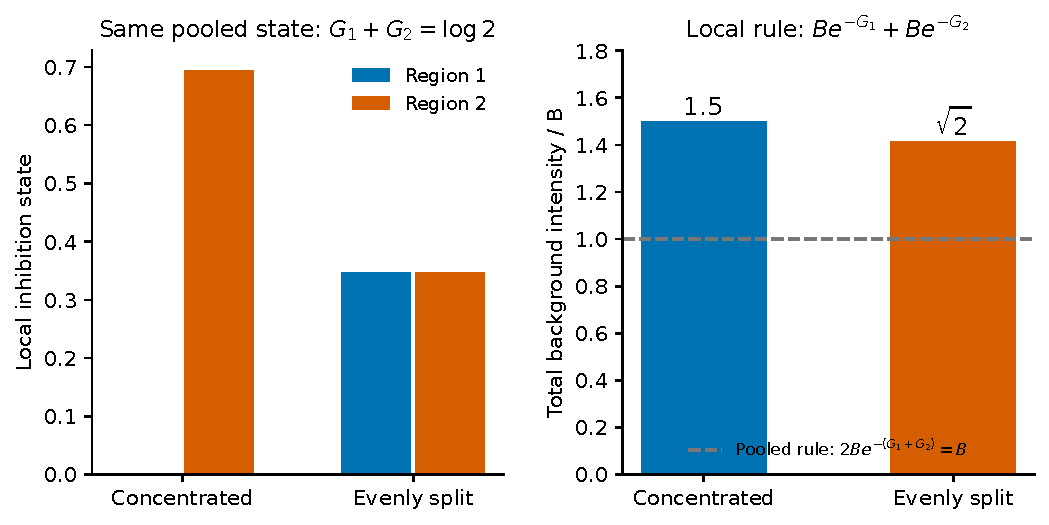
\includegraphics[width=0.85\linewidth]{pooling.pdf}
\caption{The same total depletion can have different local aggregate backgrounds. A pooled feature discards the regional allocation needed to distinguish these states. The comparison is conditional algebra, rather than an explanation of an observed predictive loss.}
\label{fig:pooling}
\end{figure}

\begin{proposition}[A conditional failure of closure under pooling]
\label{prop:regional_nonclosure}
For finitely many regions, fix $B_k\geq0$ with $B_+=\sum_kB_k>0$, nonnegative depletions $G_k$, and $\eta>0$. The local aggregate background and the pooled recipe are
\begin{equation}
 J_{\mathrm{local}}=\sum_k B_k e^{-\eta G_k},
 \qquad
 J_{\mathrm{pooled}}=B_+e^{-\eta\sum_kG_k}.
\end{equation}
The local aggregate has an effective depletion
\begin{equation}
 G_{\mathrm{eff}}=-\frac1\eta\log\left(\sum_kp_ke^{-\eta G_k}\right),
 \qquad p_k=\frac{B_k}{B_+},
 \label{eq:effective_depletion}
\end{equation}
which generally depends on the regional allocation of depletion, the background shares and $\eta$. There exist two-region backgrounds for which no function of total depletion alone, including a single rescaling of $\eta$, represents this aggregate for all regional histories. This is a failure of closure of the model class, rather than a claim that every regional configuration fails to pool.
\end{proposition}

\begin{proof}
The expression for $G_{\mathrm{eff}}$ follows by factoring $B_+$ from $J_{\mathrm{local}}$ and taking the logarithm. To show the loss of information, take two equal positive backgrounds $B$ and fix $g>0$. The histories $(G_1,G_2)=(0,g)$ and $(g/2,g/2)$ both have total depletion $g$. Their local aggregates are respectively $B(1+e^{-\eta g})$ and $2Be^{-\eta g/2}$. Their difference is
\begin{equation}
 B\bigl(1-e^{-\eta g/2}\bigr)^2>0.
\end{equation}
Every recipe using only $B_+=2B$ and $G_1+G_2=g$ gives the same value on both histories, for any common choice of its inhibition coefficient. It cannot represent both distinct local aggregates.
\end{proof}



The result permits restricted or degenerate cases in which pooling or a rescaling happens to work. It does not establish that the national recipe fails on every history, or that pooling caused the observed comparison to favour a triggering-only model. In a regional point process, adding intensities and then discarding regional labels also requires a declared filtration and a treatment of triggering across regions. Event sums assigned to spatial cells cannot supply that missing model: a joint regional likelihood includes the quiet-region compensators as well as the events. The algebra therefore motivates specifying local alternatives on a common observational target; it supplies no empirical attribution by itself.

\chapter{Likelihood, profiling and calibrated inference}\label{ch:inference}

The marked likelihood provides the common bridge from structural and visibility questions to fitted inference. It records event times, pre-event intensities, the complete observation window, and the mark factors under the same mark model. Likelihood geometry can then be separated into three questions: whether a score direction has finite second moment, whether amplitude profiling gives a well-defined finite-history optimization, and how the rejection probability of a calibrated rule responds when the generating inhibition changes.

\section{The full marked likelihood and a score bound}

For an observed marked history \((T_i,Q_i)_{i=1}^{N(T)}\), write \(G_i=G_s(T_i-)\) and \(H_i=H_e(T_i-)\), so the event at \(T_i\) is excluded from both. With the common mark density \(p_Q\),
\begin{equation}
\ell(\vartheta,\eta)
=
\sum_{i=1}^{N(T)}
\log\left\{B(T_i)e^{-\eta G_i}+nH_i\right\}
-\int_0^T\left\{B(t)e^{-\eta G_s(t)}+nH_e(t)\right\}\dif t
+\sum_{i=1}^{N(T)}\log p_Q(Q_i).
\label{eq:full-likelihood}
\end{equation}
Every event term uses its pre-event stress and trigger history, the time integral covers the full horizon, and no first event is deleted. The mark sum belongs to the full likelihood. The first two terms form its event-time contribution, evaluated on the observed marked history; they are not the marginal time-only likelihood. The mark sum cancels in a contrast only when both candidates evaluate the same marks under the same mark law and support; it is constant in ground-rate coordinates when that mark law is held fixed. Ground-rate equality without equality of mark laws is insufficient for equality of marked likelihoods. The likelihood is conditioned on the declared starting history, rather than on the observed count.

For example, let a magnitude excess \(Q\ge0\) have exponential density \(\beta e^{-\beta Q}\), and let
\[
\kappa(Q)=(1-r)e^{r\beta Q},\qquad 0\le r<1.
\]
Then \(\E \kappa=1\), and the raw triggering amplitude is
\(n(1-r)e^{r\beta Q}\). Changing \(\beta\) while holding \(r\) fixed changes both the future mark distribution and the raw productivity exponent. To preserve a raw law \(C e^{cQ}\) on the observed history under a changed \(\beta'\), one must instead use
\[
r'=c/\beta',\qquad n'=C/(1-r'),
\]
subject to \(\beta'>c\) and the branching constraints. This can preserve the event-time likelihood contribution evaluated on the observed marked history; it does not preserve the full marked law. A mark-only estimate from a training prefix is also not automatically the joint marked-process maximum-likelihood estimate, since the ground-rate term can depend on \(\beta\) through productivity.

For fixed nuisance parameters, the inhibition score is
\begin{equation}
U_\eta=\ell_\eta
=\int_0^T
-\frac{B(t)e^{-\eta G_s(t)}G_s(t)}
{B(t)e^{-\eta G_s(t)}+nH_e(t)}
\left\{\dif N(t)-\lambda_\eta(t)\dif t\right\}.
\label{eq:eta-score}
\end{equation}
At \(\eta=0\), this is the score for the declared boundary direction, with the ordinary Hawkes law as reference. The next bound shows that raw heavy-tailed marks need not imply an infinite variance for this particular intensity-weighted score.

\begin{proposition}[Restricted finite score variance]
\label{prop:score_bound}
On \([0,T]\), with empty initial history and \(\eta\geq0\), let \(0<B(t)\le B_{\max}<\infty\), \(n>0\), let \(\kappa>0\) almost surely with \(\E \kappa=1\), and let \(h_e(u)>0\) for \(0\le u\le T\). Assume the same parents contribute to \(G_s\) and \(H_e\), with nonnegative \(g\) and \(\Phi_s\), finite mean event count, \(C_T=\int_0^T\Phi_s(u)^2/h_e(u)\,\dif u<\infty\), and \(m=\E [g(Q)^2/\kappa(Q)]<\infty\). Then the score \eqref{eq:eta-score} is square integrable and its predictable variance is
\[
\E _\eta U_\eta^2
=
\E _\eta\int_0^T
\frac{(B e^{-\eta G_s}G_s)^2}{\lambda_\eta}\,\dif t
\le
\frac{B_{\max}^2}{n}C_T\,\E _\eta N(T)m<\infty.
\]
\end{proposition}

\begin{proof}
When \(H_e(t)>0\), weighted Cauchy--Schwarz with weights \(\kappa(Q_i)h_e(t-T_i)\) gives
\[
G_s(t)^2
\le
H_e(t)\sum_{T_i<t}
\frac{g(Q_i)^2}{\kappa(Q_i)}
\frac{\Phi_s(t-T_i)^2}{h_e(t-T_i)}.
\]
When \(H_e=0\) there are no preceding parents and both displayed quantities are zero. Since \(\lambda_\eta\ge nH_e\) and \(B e^{-\eta G_s}\le B_{\max}\),
\[
\frac{(B e^{-\eta G_s}G_s)^2}{\lambda_\eta}
\le
\frac{B_{\max}^2}{n}
\sum_{T_i<t}
\frac{g(Q_i)^2}{\kappa(Q_i)}
\frac{\Phi_s(t-T_i)^2}{h_e(t-T_i)}.
\]
Integrating and applying Tonelli's theorem bounds the expected bracket by
\[
\frac{B_{\max}^2}{n}C_T
\E _\eta\sum_{T_i<T}\frac{g(Q_i)^2}{\kappa(Q_i)}.
\]
Fresh marks are drawn independently after acceptance, so the last expectation equals \(\E _\eta N(T)m\), although marks may influence future event counts. The stochastic-integral score is therefore an \(L^2\) martingale with the stated variance.
\end{proof}

Raw \(\E  g^2\) or \(\E \kappa^2\) may be infinite while the intensity-weighted ratio has finite moment. Positive \(n\) and matched triggering parents supply the required comparison history; the bound is not uniform as \(n\downarrow0\) or as the kernel-ratio integral grows.

\paragraph{Example at the synthetic mark parameters.}
For \(Q\sim\operatorname{Exp}(\beta)\),
\(g(Q)=e^{\gamma(Q-1)}\) and \(\kappa(Q)=(1-r)e^{r\beta Q}\),
where \(\gamma=\tfrac34\log 10\) is the local stress-mark exponent,
distinct from the auxiliary response gain in Chapter~\ref{ch:stability}.
The magnitude-six reference factor is included in \(g\); the outer
branching coefficient \(n\) is not included in \(\kappa\). Then
\[
  \E\!\left[\frac{g(Q)^2}{\kappa(Q)}\right]
  =\frac{e^{-2\gamma}}{1-r}
    \frac{\beta}{\beta(1+r)-2\gamma},
  \qquad \beta(1+r)>2\gamma.
\]
At the declared synthetic values \(\beta=2.849401764894274\) and \(r=0.7\),
the denominator is approximately \(1.390105\), giving
\(m\approx0.216065\). Although both first moments are finite,
\(2\gamma>\beta\) and \(2r\beta>\beta\), so
\(\E[g(Q)^2]=\E[\kappa(Q)^2]=\infty\).
The finite weighted moment verifies this mark condition in Proposition~\ref{prop:score_bound},
not all its other hypotheses by itself. The positive-triggering,
matched-parent, finite-horizon and kernel-ratio conditions remain essential to that bound;
the bound is not uniform near the simultaneous zero boundary, and
no joint Fisher-information, central-limit or Wilks conclusion follows.

At the simultaneous boundary \(n=\eta=0\), the conclusion can fail. Take a constant Poisson background \(B>0\), marks \(Q\sim\operatorname{Exp}(\beta)\), and \(g(Q)=e^{\gamma(Q-1)}\) with \(\gamma<\beta\le2\gamma\). The first stress-mark moment is finite while the second is infinite. For one exponential relaxation mode of rate \(k>0\), the resulting positive shot noise has a stationary version of mean \(B\E g/k\); copies with the same future points and marks have differences that decay exactly as \(e^{-kt}\). Thus a first-moment stable state process is compatible with the following score irregularity. On the positive-probability event of exactly one event at \(S<T\), the pre-event stress is zero and the score contribution has the form
\[
U_0=g(Q)\int_S^T B(t)\Phi_s(t-S)\,\dif t.
\]
The fresh mark is independent of that event configuration, and the integral is strictly positive on a positive-probability set of \(S\). Hence the score has infinite second moment. At positive \(\eta\), even with \(n=0\),
\[
\frac{(G_sB e^{-\eta G_s})^2}{\lambda_\eta}
\le B G_s^2e^{-\eta G_s}
\le\frac{4B}{e^2\eta^2},
\]
so integrable \(B\) controls the score bracket without a raw second mark moment. This regularization is not uniform as \(\eta\downarrow0\) and does not establish null-boundary asymptotic theory.

Finite score variance alone is not a central limit theorem. It also does not establish differentiability in quadratic mean for the full searched model or a regular information matrix at the boundary. The pathwise second derivative contains terms whose expectations may fail even when the martingale-score bracket is finite.

\section{Nuisance projection and local information}

Suppose the relevant scores are square integrable. Define the ensemble inner product
\[
\langle f,h\rangle_0
=
\E _0\int_0^T\lambda_0(t)f(t)h(t)\,\dif t.
\]
For a nuisance parameter \(\zeta\), the score integrand is
\(f_\zeta=\partial_\zeta\lambda_0/\lambda_0\). If the nuisance scores span a closed subspace, the residual after projecting \(f_\eta\) onto that subspace is the efficient-score integrand. In finite nonsingular notation,
\[
I_{\eta\mid\zeta}
=
I_{\eta\eta}-I_{\eta\zeta}I_{\zeta\zeta}^{-1}I_{\zeta\eta}
\le I_{\eta\eta}.
\]
When nuisance scores are redundant, a generalized inverse and its range condition replace the ordinary inverse.

This projection gives a quantitative meaning to masking by fitted background and triggering. Slowly varying depletion can resemble a background trend, while post-event depletion can resemble a triggering scale or productivity. It also shows why effective information is an ensemble object: it requires integrability and a reference law, not merely the algebra of one fixed path. At \(\eta=0\), the information contributed by an independently parameterized stress-kernel direction is zero, because
\(\partial_\theta\lambda=-\eta B e^{-\eta G_s}\partial_\theta G_s\).
An \(O(\eta^2)\) information statement away from zero requires a justified uniform moment bound for that derivative; the zero first derivative alone is not enough.

A related calculation can be made on one fixed reference path without the ensemble expectation. For \(B=\exp(a+dx)\), the four null log-intensity directions are
\[
s_a=\frac B{\lambda_0},\quad
s_d=\frac{xB}{\lambda_0},\quad
s_n=\frac{H_e}{\lambda_0},\quad
s_\eta=-\frac{BG_s}{\lambda_0}.
\]
The realized Gram matrix \(J_{ij}=\int_0^T\lambda_0s_is_j\,\dif t\) is positive semidefinite. Its residual inhibition norm after projecting on \((s_a,s_d,s_n)\) is the minimum of
\(\int\lambda_0(s_\eta-b_as_a-b_ds_d-b_ns_n)^2\dif t\).
If \(G_s=c_0+c_1x+c_2H_e/B\), that residual is exactly zero. This algebra explains how depletion can resemble a fitted level, trend and triggering component.

On two frozen reference paths, the archived residual/raw squared-norm ratios were approximately \(10.82\%\) and \(3.26\%\). These are two realized-path projections, rather than estimates of ensemble Fisher information. The paths and their calibrations differ; their ordering does not establish that greater exposure reduces expected information. Additional score directions can only reduce the residual for the same path and inner product, but no power decomposition follows from that projection fact.

\section{Conditional amplitude profiling}

Fix one observed marked history and fix the trend coefficient \(d\) and inhibition \(\eta\). Put
\[
q_i=\exp\{d x(T_i)-\eta G_i\},
\qquad
c_i=nH_i,
\qquad
J=\int_0^T\exp\{d x(t)-\eta G(t)\}\,\dif t,
\]
and let \(A=\exp(a)\) with \(A\in[L,U]\), where \(L=e^{-12}\) and \(U=1\). The negative event-time contribution to the joint marked log-likelihood, omitting the common mark constant and writing \(K\) for the full-window triggering compensator, is
\begin{equation}
F(A;d,\eta)=AJ+nK-\sum_{i=1}^{N}\log(Aq_i+c_i).
\label{eq:amplitude-objective}
\end{equation}
The full horizon and all pre-event intensities are retained. The mark factors in \eqref{eq:full-likelihood} are constant in these fitted coordinates under the common mark model.

\begin{proposition}[Conditional amplitude profile]
\label{prop:amplitude}
Assume a finite history and finite event features and parameters. Let every \(c_i\ge0\), let \(K\) be finite, and require \(0<J<\infty\). The specified finite-mode observation window satisfies these conditions when \(x\) is bounded and all recorded marks are finite. Then \eqref{eq:amplitude-objective} has a unique minimizer on \([L,U]\):
\begin{enumerate}
\item if \(F_A(L)\ge0\), the minimizer is \(L\);
\item otherwise, if \(F_A(U)\le0\), the minimizer is \(U\);
\item otherwise, the unique interior root of the continuous strictly increasing \(F_A\) is the minimizer.
\end{enumerate}
If \(N=0\), the unique minimizer is \(L\).
\end{proposition}

\begin{proof}
Ordinary finite-sum differentiation gives
\[
F_A=J-\sum_{i=1}^{N}\frac{q_i}{Aq_i+c_i},
\qquad
F_{AA}=\sum_{i=1}^{N}
\left(\frac{q_i}{Aq_i+c_i}\right)^2.
\]
For \(N\ge1\), \(q_i>0\), so \(F_{AA}>0\) and \(F_A\) is strictly increasing and continuous on the compact interval. If its endpoint values place zero inside the interval, it has one root, and the sign change from negative to positive identifies that root as the unique minimizer; endpoint cases place the minimizer at the corresponding boundary. If \(N=0\), then \(F(A)=AJ+nK\) is strictly increasing because \(J>0\), so the lower endpoint is the unique minimizer.
\end{proof}

The amplitude result is a finite-history optimization fact, not a global fit certificate. Convexity in \(A\) does not make the profiled surface \(V(d,\eta)=F(A_*(d,\eta);d,\eta)\) convex in \((d,\eta)\). A finite grid or local search establishes only its declared numerical search outcome.

For \(a=\log A\), set \(p_i=Aq_i/(Aq_i+c_i)\). Then
\[
g(a)=F_a=AJ-\sum_i p_i,
\qquad
g'(a)=AJ-\sum_i p_i(1-p_i),
\]
and \(g\) need not be monotone even though \(F_A\) is increasing in \(A\). A bracketing method for \(a\) can rely on continuity and endpoint signs, not on monotonicity of \(g\). At an interior root the exact balance is
\[
AJ=\sum_i p_i.
\]
The curvature identity in log amplitude is
\[
F_{aa}=\sum_i p_i^2+R,
\qquad
R=AJ-\sum_i p_i.
\]
Thus at the balanced root, the negative log-likelihood satisfies
\(F_{aa}=\sum_i p_i^2\), while the log-likelihood \(\ell=-F\) satisfies
\(\ell_{aa}=-\sum_i p_i^2\). At an approximate root, the balance residual \(R\) must be added to \(\sum_i p_i^2\); it is not exact curvature at that numerical point. In an interior fixed-\(d\) region, profile differentiation also gives
\[
V_d=AJ_x-\sum_i x(T_i)p_i,
\qquad
V_\eta=-AJ_G+\sum_i G_ip_i,
\]
where \(J_x\) and \(J_G\) integrate \(x(t)\) and \(G(t)\) against the background weight. Here \(J_x=\int_0^Tx(t)e^{dx(t)-\eta G(t)}\dif t\) and \(J_G=\int_0^TG(t)e^{dx(t)-\eta G(t)}\dif t\). At fixed \(d\), implicit differentiation in an interior-amplitude region gives

\[
\frac{\partial a_*}{\partial\eta}
=\frac{AJ_G-\sum_iG_ip_i(1-p_i)}{\sum_i p_i^2}.
\]
The numerator has no universal sign. An amplitude curve that also refits trend has a different total derivative. The identity \(AJ=\sum_i p_i\) equates integrated fitted background with event-wise background mixture weights; these weights are not observed physical parent labels or a stationary balance law. With empty prehistory and positive background, the first event has \(c_1=0\), so \(p_1=1\). No initial quiet interval or first event can be discarded from this argument.

These are local envelope and implicit formulas. Active endpoint transitions require one-sided treatment, and none of them implies that every starting point reaches the global profile minimum.

Stable evaluation also matters for the conditional proof. In logarithmic coordinates compute \(\log\lambda_i\) by a log-sum-exp of \(a+\log q_i\) and \(\log c_i\). When \(c_i=0\), the mathematically positive background gives \(p_i=1\), even if exponentiating \(\log q_i\) underflows. A numerical zero is not evidence that the exact objective is flat. The same amplitude algebra holds with positive quadrature weights, but agreement between quadrature orders at selected points is a numerical sensitivity check rather than a rigorous global integration bound.

\section{Boundary hypotheses and calibration}
\label{sec:boundary_calibration}

Feedback detection and testing equality of memories are different tasks. The first compares \(\eta=0\) with an active alternative; the second compares shared and separate stress/trigger families while permitting inhibition. At zero feedback, an independently varied stress-kernel parameter disappears from the observed law. Together with the one-sided constraint \(\eta\ge0\), this produces a nonregular null: there is a nuisance parameter present only under the alternative. A fixed-kernel boundary formula cannot automatically calibrate a maximization over stress kernels and fitted nuisances. The general difficulty is discussed by \citet{Davies1977}; the regularity conditions of boundary likelihood theory, including those in \citet{SelfLiang1987}, need their own verification here.

A calibration recipe must match the complete statistic actually computed. Under a fitted null, this means simulating new marked catalogues, refitting the allowed nuisance parameters under both candidates, repeating the declared kernel search and using the same failure and selection rules. A reference distribution for one nuisance block cannot be substituted for another. Such a plug-in procedure is a proposed finite-sample method; the present score bounds do not prove its uniform validity over a composite null or near weak identification. Non-rejection of shared memory cannot confirm that restriction without evidence that meaningful separate-memory alternatives are distinguishable.

The distinction between supplied and estimated nuisances is equally substantive. A likelihood ratio between two fully specified laws addresses a simple testing problem. A composite null can change its background and other permitted parameters, admitting alternative explanations that the simple null excludes. Superior calibrated detection with supplied generating values therefore does not measure purely avoidable fitting inefficiency. It combines different statistical questions with different procedures; neither an arbitrary optimizer improvement nor fixing real-data nuisance values without justification is guaranteed to recover the supplied-law performance.

\section{Response of a calibrated fixed-rule test}

Calibrated inference starts with a complete-data decision rule rather than with a particular fitted parameter value. Let \(I(\mathcal H)\in\{0,1\}\) be a fixed bounded measurable rejection indicator defined on every admissible marked history. The reference bank, tuning and model-selection procedure, critical threshold, treatment of empty histories, and any auxiliary randomization law are fixed independently of the true generating inhibition. The rule may estimate nuisances or select a model from the data, because these operations are part of the same measurable mapping from history to \(\{0,1\}\); what is held fixed is the rule as the generating \(\eta\) varies. Define
\[
p(\eta)=\E _\eta I(\mathcal H).
\]

\begin{proposition}[Positive-inhibition response of a fixed rule]
\label{prop:power_response}
Fix empty history, a common fresh mark law with finite nonnegative transforms, \(\E \kappa=1\), \(0\le n<1\), nonnegative kernels bounded on the finite window with normalized \(h_e\), and a deterministic nonnegative background with \(\mathcal B=\int_0^TB(t)\dif t<\infty\). Hold all these generating nuisances fixed as \(\eta\) varies. Then \(p(\eta)\) is continuously differentiable for \(\eta>0\), and
\[
p'(\eta)=\E _\eta[I(\mathcal H)S_\eta]
=\mathrm{Cov}_\eta(I(\mathcal H),S_\eta).
\]
Moreover,
\[
|p'(\eta)|
\le
\frac{2\sqrt{\mathcal B\,p(\eta)(1-p(\eta))}}{e\eta}
\le
\frac{\sqrt{\mathcal B}}{e\eta}.
\]
\end{proposition}

\begin{proof}
Let \(P_0\) be the noninhibited Hawkes law. Its mean count is at most \(\mathcal B/(1-n)\), and it dominates each inhibited construction. On a finite path the likelihood ratio is
\[
L_\eta=\exp\left\{\int_0^TB(1-e^{-\eta G_s})\dif t\right\}
\prod_i\frac{Be^{-\eta G_i}+nH_i}{B+nH_i}\le e^{\mathcal B}.
\]
At actual event times the reference intensity is positive almost surely; where both intensities vanish away from events, set their likelihood ratio to one. The stopped density martingale is uniformly bounded and hence defines the changed law. Its score \(S_\eta=\partial_\eta\log L_\eta=U_\eta\) satisfies
\[
\E _\eta S_\eta=0,\qquad
\E _\eta S_\eta^2\le\frac{4\mathcal B}{e^2\eta^2},
\]
by the positive-inhibition bracket bound, without a raw stress-mark second moment.

For clarity, write
\[
\begin{aligned}
 \mathcal B&=\int_0^T B(t)\,\dif t,
 &J_\eta&=\int_0^T B(t)(1-e^{-\eta G_s(t)})\,\dif t,\\
 q_i(\eta)&=\frac{B_i e^{-\eta G_i}+c_i}{B_i+c_i},
 &c_i&=nH_i\geq0,
\end{aligned}
\]
where $B_i=B(T_i)$ and $G_i,H_i$ are the pre-event features. Then
$L_\eta=e^{J_\eta}\prod_iq_i(\eta)$, with $0\leq q_i\leq1$ and
$0\leq J_\eta\leq\mathcal B$. At actual reference-law events
$B_i+c_i>0$ almost surely. On a compact positive interval
$\eta\in[\eta_-,\eta_+]$, direct differentiation gives
\[
 |q_i'(\eta)|
 =\frac{B_i}{B_i+c_i}G_i e^{-\eta G_i}
 \leq\frac{1}{e\eta_-},
 \qquad
 |J_\eta'|\leq\frac{\mathcal B}{e\eta_-}.
\]
The product rule, without division by any $q_i$, therefore yields
\[
\begin{aligned}
 |\partial_\eta L_\eta|
 &\leq e^{J_\eta}\left(
 |J_\eta'|\prod_iq_i+
 \sum_i |q_i'|\prod_{j\ne i}q_j\right)\\
 &\leq\frac{e^{\mathcal B}(\mathcal B+N(T))}{e\eta_-}.
\end{aligned}
\]
The same bound applies to $|\partial_\eta(L_\eta I)|$ for the fixed bounded
indicator. It is integrable under the reference law because
$\E _0N(T)\leq\mathcal B/(1-n)$. The bound is for the derivative of
$L_\eta$, not its logarithm. The finite-path derivative is continuous in $\eta$. Dominated convergence gives
\(p'(\eta)=\E _0[I\partial_\eta L_\eta]=\E _\eta[IS_\eta]\).
No derivative of the data-dependent fitted outputs is taken: \(I\) is the same mapping on every history. The mean-zero score gives the covariance identity. Cauchy--Schwarz with \(\mathrm{Var}(I)=p(1-p)\) gives the stated bounds.
\end{proof}

The covariance has no proved sign. Stronger generating inhibition need not increase detection probability for a particular calibrated rule. Positive \(\eta\) gives local differentiability and moment control, not monotonic power and not control as \(\eta\downarrow0\). Unknown, failed, capped, or otherwise unresolved computational outcomes remain unknown; they must not be recorded as nonrejections. Conditioning on completed cases estimates a different functional from the unconditional \(p(\eta)\) defined by the fixed rule.

The proposition also does not compare a simple hypothesis with a known generating law to a composite hypothesis whose nuisances are fitted. Those are different operating characteristics, with different permitted null explanations and decision rules. An oracle that knows the nuisance values and a composite rule that estimates them are not the same test function, so their performance gap is not by itself pure fitting waste.

\section{Scope and unresolved inference}

Taken together, the results separate four questions. Exact marked-law equality shows that zero feedback leaves a separately varied stress kernel unidentified; the restricted active-inhibition experiment can identify the inhibition parameter and kernel in an idealized full-law sense; the restricted score can remain square integrable even when raw mark moments diverge; and a calibrated fixed rule has a local covariance response at positive inhibition. Amplitude profiling adds a unique conditional optimization in \(A\), while leaving the remaining trend--inhibition surface without a global certificate.

These statements do not imply a Wilks law, a general Fisher-information theorem, likelihood-ratio asymptotics at \(\eta=0\), uniform validity near the boundary, a necessary detection threshold, or a finite-sample power result. They also provide no new numerical evidence and do not replace a specified calibration procedure by a general asymptotic claim. The unresolved inference is therefore explicit: structural identification in a restricted family is not practical detectability; finite score variance is not a distributional approximation; conditional amplitude uniqueness is not global identifiability; and a signed response formula for a fixed rule is not a theorem that stronger inhibition creates a more powerful test.

\chapter{Design and interpretation of the finite-history experiment}
\label{ch:design}

This chapter specifies the finite-history experiment used to study detection of the diagnostic inhibition term. The quantity of primary interest is a diagnostic inhibition parameter, \(\eta\), not the physical loading parameter of the original process model. The distinction is substantive. Within the diagnostic family, a positive \(\eta\) suppresses the background contribution after the specified history feature is represented. It does not identify the original physical loading parameter, nor does it establish a unique physical mechanism. The experiment is therefore an inference study about a class of fitted laws, not a reconstruction of a complete physical loading history.

The synthetic construction is model-correct relative to the laws it generates: histories are produced from the stated marked point-process model, evaluated under that model, and compared without introducing an external observation model. Geography, changing observation practices, and missing parents are deliberately omitted. Consequently, agreement or disagreement among procedures on these histories measures behavior within a specified filtration and law class. It cannot by itself establish that the same procedures are adequate for a catalogue affected by spatial heterogeneity, reporting changes, or genealogical incompleteness.

\section{The diagnostic law and its history}

For a history \(\mathcal H_t\), let
\begin{equation}
\lambda_\eta(t)
=
\exp\!\left\{a+d\left(\frac{2t}{T}-1\right)\right\}
\exp\{-\eta G_s(t)\}
+
nH_e(t),
\label{eq:experiment-intensity}
\end{equation}
where
\[
B(t)
=
\exp\!\left\{a+d\left(\frac{2t}{T}-1\right)\right\}.
\]
Here \(a\) controls the background level, \(d\) the linear trend in transformed time, \(n\) the additive triggering scale, and \(\eta\) the diagnostic inhibition of marked stress memory. The feature \(G_s(t)\) is a nonnegative marked stress-memory feature, while \(H_e(t)\) is a normalized marked triggering feature. The interpretation of \(\eta\) is conditional on the represented triggering process and on the specified background: it is an attenuation of the first term in \eqref{eq:experiment-intensity}, not a declaration that the physical process is governed by an equivalent coefficient.

Both \(G_s\) and \(H_e\) are functions of the strictly earlier history. If event \(i\) has time \(t_i\) and mark \(m_i\), the predictable intensity used for that event is \(\lambda_\eta(t_i-)\). The mark \(m_i\) affects later stress memory and later triggering but cannot affect the intensity immediately before its own occurrence. This timing convention prevents circular use of the event being evaluated and is essential to the likelihood interpretation below.

The numerical kernels are positive normalized finite spectral mixtures. They represent the stress and triggering responses with a finite number of modes rather than by evaluating the exact Mittag--Leffler kernel. In the shared implementation, the kernel scale parameters are \(\alpha=0.5\) and \(\tau=1\), and the normalized mixture comprises \(195\) modes. Although the modes may approximate a long-memory response, the finite mixture is itself the implemented model. For magnitude excess \(m_i=M_i-M_0\), the implemented features are
\begin{align}
 G_s(t)&=\sum_{t_i<t} e^{\gamma(m_i-1)}\Phi_s(t-t_i),
       &\gamma&=\tfrac34\log 10,\\
 H_e(t)&=\sum_{t_i<t}(1-r)e^{\beta r m_i}h_e(t-t_i).
 \label{eq:diagnostic-features}
\end{align}
The relaxation kernel has the form \(\Phi_s(u)=\sum_qw_qe^{-\rho_qu}\), with positive weights summing to one. The corresponding triggering density is \(h_e(u)=\sum_qv_q\zeta_qe^{-\zeta_qu}\), with positive weights summing to one and positive rates. Thus \(\Phi_s(0)=1\) and \(\int_0^\infty h_e(u)\,\dif u=1\). Sharing the relaxation parameters means using a common survival kernel and its negative derivative as the triggering density, rather than setting the two functions equal. The stress-mark normalization is the declared magnitude-six reference when \(M_0=5\). These formulas are explicit in \href{https://github.com/Drefetr/InhibitoryEarthquakeModels/blob/3e76a174cf4f58ce601c6c9640c4d0c11168813f/engine/iteration_20/code/restricted_history.py}{public restricted-history implementation} (\texttt{S10}) and \href{https://github.com/Drefetr/InhibitoryEarthquakeModels/blob/3e76a174cf4f58ce601c6c9640c4d0c11168813f/engine/iteration_27/code/adequacy.py}{public observed implementation} (\texttt{S17}). Conclusions therefore apply to the finite mixture that was used, not automatically to every exact infinite-mode limit.

\paragraph{Finite spectral recipe.}
For \(0<\alpha<1\) and the dimensionless rate variable $r$, the continuous representation
\citep[Eqs.~(2.12)--(2.13)]{Mainardi2014} is
\[
 E_\alpha(-t^\alpha)=\int_0^\infty e^{-rt}K_\alpha(r)\,\dif r,
 \qquad
 K_\alpha(r)=\frac{\sin(\pi\alpha)}{\pi}
 \frac{r^{\alpha-1}}{r^{2\alpha}+2r^\alpha\cos(\pi\alpha)+1}.
\]
Writing $r=e^v$ gives the log-rate density
\[
 K_\alpha(e^v)e^v=
 \frac{\sin(\pi\alpha)}{2\pi\{\cosh(\alpha v)+\cos(\pi\alpha)\}}.
\]
For the scaled relaxation $E_\alpha(-(t/\tau)^\alpha)$, the rates are
$e^v/\tau$. The following finite rule applies trapezoidal weights on the
stated log-rate grid, halves its endpoints, truncates and renormalizes.
The continuous representation and this numerical discretization are distinct;
the citation does not provide a universal likelihood- or inference-error bound.
The generating relaxation uses log rates \(v_j=0.4j\), \(j=-97,\ldots,97\), and rates \(\rho_j=e^{v_j}/\tau\) in days\(^{-1}\), with \(\alpha=0.5\) and \(\tau=1\) day. Before normalization its weights are
\[
 \widetilde w_j=\frac{0.4\sin(\pi\alpha)}{2\pi\{\cosh(\alpha v_j)+\cos(\pi\alpha)\}},
\]
with both endpoint weights halved, then \(w_j=\widetilde w_j/\sum_k\widetilde w_k\). More generally the implemented endpoint index is
\[
 J=\left\lceil\frac{1}{s}\max\left\{\frac{\log4}{\alpha},
 \frac{\log[4\sin(\pi\alpha)/(\pi\alpha\varepsilon)]}{\alpha}\right\}\right\rceil,
 \qquad s=0.4,\quad\varepsilon=10^{-8}.
\]
Thus the 195-mode count specifies the generating case, while candidate \(\alpha=0.7\) uses 137 modes with the same spectral rule. The machine-readable methods supplement supplies the rates and normalized weights. The finite triggering density remains \(h=-\Phi'\); its finite value at zero does not reproduce the exact fractional singularity.


Marks are generated with excess density
\[
f_\beta(m)=\beta e^{-\beta m},\qquad m>0,
\]
with \(\beta=2.849401764894274\). The normalized productivity factor is
\[
(1-r)e^{\beta r m},\qquad r=0.7.
\]
This normalization gives unit mean productivity at the reference scale and makes the mark contribution positive. The exponential excess itself has finite moments. It is the exponential stress and productivity transforms that have finite first but infinite second moments at the declared parameters. That feature motivates bounded-indicator simulation checks rather than variance formulas or finite-information shortcuts based only on the raw marks.

\section{Generating histories and evaluating both laws}

The main generating experiment has duration \(T=24394\) days, begins with an empty prehistory, and produces random event counts. Counts are not conditioned on a target total; in particular, the design does not condition on a 913-event count. The generating nuisance parameters include
\[
a=-4.162108473051707,\qquad
d=0.23211265877958467,\qquad
n=0.5017751599706763,
\]
and the main diagnostic value is
\[
\eta=0.4885010300470942.
\]
The null experiment sets \(\eta=0\) while retaining the generating nuisance values in the null law. This is a comparison between a marked process with stress inhibition and a marked process without that inhibition, not a comparison against a law with triggering or marks removed.

\paragraph{Simulation and event clock.}
The simulator starts both modal states at zero. At each proposal it samples an exponential wait with envelope \(e^{a+|d|}+\sum_qw_qE_q\), where \(E_q\) is the current excitation state, advances and decays both modal states, and accepts with probability equal to the new predictable intensity divided by that envelope. Nonnegative inhibition bounds the background by \(e^{a+|d|}\), and excitation decays between events. Only after acceptance is a fresh exponential excess mark drawn; its productivity and stress increments then update future states. Proposals reaching the horizon add no event. The accepted clock retains the legacy compensated binary64 projection and the exact Decimal sum of sampled binary64 waits at precision 1600, together with residual coordinates and positive relative event gaps. Projected ties are retained without jitter or resampling; paired-clock likelihood evaluation uses those gaps. Unrepresentable waits, mark-transform overflow and resource caps remain explicit unresolved cases, with restart state retained.


For observed event times \(t_i\) and marks \(m_i\), the marked point-process log likelihood is
\begin{equation}
\ell(\vartheta,\eta;\mathcal H_T)
=
\sum_{i:t_i\le T}\log\lambda_\eta(t_i-)
-
\int_0^T\lambda_\eta(t)\,\dif t
+
\sum_{i:t_i\le T}\log f_\beta(m_i).
\label{eq:marked-likelihood}
\end{equation}
Evaluation uses the full predictable intensity and the full integral, including quiet exposure before, between, and after events and the terminal interval up to \(T\). It is not a count-conditional likelihood on the event times alone. When the same mark density is held fixed for both laws, the mark terms in \eqref{eq:marked-likelihood} cancel in their difference. They are present in both likelihoods; their cancellation is an algebraic consequence of the common mark law, not an omission of marks from the model.

Two comparison designs are distinguished. An oracle signed log-likelihood ratio compares two fully supplied laws. A fitted generalized statistic instead permits separate null and alternative optimizations over the nuisance parameters allowed by each procedure. The oracle therefore has additional information: it knows nuisance values that an estimation procedure must recover. This changes a simple-law comparison into a composite-law task. A contrast such as \(100\%\) detection for the known-law procedure versus roughly \(38\%\) for a fitted procedure is not, by itself, evidence of avoidable numerical inefficiency, nor does it establish the power of a hypothetical oracle for the composite problem. Estimating nuisance changes both the test statistic and its null distribution. Each procedure consequently requires its own reference calibration. In symbols, the oracle uses the signed contrast
\begin{equation}
 L_{10}=\ell(\vartheta_\star,\eta_\star;\mathcal H_T)
        -\ell(\vartheta_\star,0;\mathcal H_T),
 \label{eq:oracle-statistic}
\end{equation}
whereas a fitted procedure uses its selected maxima to form
\begin{equation}
 D=2\left\{\widehat\ell_1-\widehat\ell_0\right\}.
 \label{eq:fitted-statistic}
\end{equation}
The hats denote the declared finite fitting recipe, rather than a proof that a global maximum has been found. The oracle contrast need not be nonnegative; a fitted statistic with an exact eligible null floor is nonnegative. Their numerical scales and critical values cannot be exchanged.

\section{Reference calibration and inferential scope}

For each historical matched-law method described here, the null calibration uses \(999\) reference null history identifiers and a separate bank of \(1{,}000\) null query histories. The same reference identities are reused across methods, but each method fits and scores its own statistic on those histories. The \(150\) stronger alternative histories are also held in common across procedures. Reference histories are not scored as queries. For a query statistic \(D_q\), the reported rank probability is
\begin{equation}
p=\frac{1+\sum_{j=1}^{999}\mathbf 1\{D_j\ge D_q\}}{1000},
\qquad
\text{reject if }p\le 0.05.
\label{eq:rank-p}
\end{equation}
All ties count through the indicator, with no random tie breaking or exclusion. The add-one term and the denominator of \(1{,}000\) make the query effectively one member of a rank set containing \(999\) calibration references.

The reported summaries condition on the realized reference banks and generating law. For a procedure fixed in advance whose reference and query histories are exchangeable under the null, the rank rule has the usual finite-sample conservativeness of a Monte Carlo rank test. That ideal argument is not retrospective proof for a procedure selected and reused during the research process. Adaptive selection followed by scoring can alter both the statistic and the comparison being calibrated. The reported Clopper--Pearson intervals are nominal exact binomial summaries under fixed-bank, fixed-procedure and independent-query assumptions. They describe Monte Carlo uncertainty in query outcomes, rather than conditioning away those outcomes. They do not resample the reference bank, the generator, or the adaptive procedure-selection process. Similar realized null rejection rates therefore do not prove equal test size uniformly over a composite null.

The null value \(\eta=0\) lies on the boundary of the permitted nonnegative parameter space. The usual interior-parameter Wilks argument does not apply directly. This study uses empirical matched-null calibration rather than asserting a chi-squared reference law. The inferential calculations are based on the separately calibrated procedures and their realized reference distributions. Because each rejection decision is a bounded indicator, conditional Monte Carlo standard errors remain meaningful even when individual marked histories are heavy tailed. This does not imply that a finite joint Fisher information exists for the fitted model.

\section{Numerical controls and completed evidence}

The evaluation retains the full event clock, including extreme histories, rather than replacing generated histories with summaries. Required optimizer starts must resolve; an unresolved calculation stopped at a cap is recorded as unknown and is never converted into a non-rejection. Selected-point likelihood and intensity comparisons were checked across integration orders and backends, and direct likelihood contrasts were used where possible to reduce cancellation between nearly equal large integrals. Numerical envelopes serve as sensitivity controls for these calculations. They are not a universal quadrature bound and do not establish global maxima for an optimization.

The completed historical oracle, supplied-nuisance, estimated-background and level-only evaluations each retain all \(2{,}149\) declared histories. No failed or extreme history is removed to obtain these denominators. This historical completeness statement does not apply to the later bounded F continuation in Section~\ref{sec:f-continuation}, which has separately reported controlled and unknown method outcomes. Reporting policies, inclusion rules, and provenance for the numerical controls are recorded in the appendix. The completed-history evaluation and its reference-calibration conventions are documented in \hyperlink{S09}{archival \texttt{S09} (not distributed)}; the matched synthetic construction and likelihood accounting are recorded in \hyperlink{S11}{archival \texttt{S11} (not distributed)}, and the final reporting structure is recorded in \hyperlink{S16}{archival \texttt{S16} (not distributed)}.

\paragraph{Procedure-specific estimation.}
The completed supplied-trigger studies hold \(n,r,\beta,\alpha_e,\tau_e\) and the stress kernel fixed. The eta-only procedure uses starts \(0\) and \(0.2\) over \(\eta\in[0,3]\). The level-and-trend procedure runs two null optimizations in \((a,d)\in[-12,0]\times[-2,2]\) and selects the better null fit. It then runs two alternative optimizations from that one fit, initialized at \(\eta=0\) and \(\eta=0.2\). Thus level-and-trend has four prescribed optimizations; the two procedures together have six. Both use L-BFGS-B with \(\mathrm{maxiter}=100\), \(\mathrm{maxls}=40\), \(\mathrm{ftol}=10^{-10}\) and \(\mathrm{gtol}=2\times10^{-6}\). Failure alone enables the same-start CPU retries (line-search limits 40 then 200), followed by bounded Powell; the supplied-trigger procedures never free \(n\). Every prescribed start must resolve, the exact matching null remains eligible, and selected order 16 values are checked independently at CPU order 32 to tolerance \(10^{-4}\).
The distinct level-only procedure supplies \(d\) and profiles \(a\in[-12,0]\) for each \(\eta\). It checks 17 equally spaced \(\eta\)-values in \([0,3]\), the saved supplied-background alternative and zero, refines strict local mesh minima, and includes an 11-point profile. Its saved eligible floors and all mandatory solver returns are retained. Complete bounds, starts, stopping and recovery rules for this procedure, the historical fuller fit and the observed predictive fits are given separately in the methods supplement; none is a claim of global optimization. The later F continuation uses a separately frozen fitting and control contract, rather than a rerun of these historical recipes.

\paragraph{Numerical integration and stable evaluation.}
The positive-gap history geometry retains initial and terminal quiet exposure. Within each event gap it inserts the offsets shorter than the gap from 23 geometric values spanning \(10^{-6}\) to \(10^5\) days and their 22 adjacent geometric means, then applies Gauss--Legendre order 16 on each subpanel. Selected controls use independent CPU order 32; the oracle refinement can require order 64. The triggering compensator uses the finite-mixture CDF, evaluated with \(-\operatorname{expm1}(-\rho_q u)\). Event log intensity uses a log-sum-exp evaluation, including an explicit zero-triggering branch. Each event reads the decayed pre-event state before adding its mark. The historical fuller search and observed search have separate parameter and recovery contracts in the companion specification.

\paragraph{Companion procedure specification.}
The portable methods supplement and machine-readable settings in \texttt{supplements/}
% Exact companion paths: supplements/methods_supplement.md; supplements/methods_settings.json
 distinguish the generating kernel, the historical fuller calibration, the supplied-trigger procedures, the level-only profile and the observed predictive search. They record estimated and supplied coordinates, bounds, starts, quadrature, recovery and unresolved availability limits at their respective accepted versions. The metadata arrays are deterministic evaluations of the documented mixture rule, not new event histories or refits.

The \href{https://github.com/Drefetr/InhibitoryEarthquakeModels/blob/3e76a174cf4f58ce601c6c9640c4d0c11168813f/paper/data/detection.json}{public detection summary} and the \hyperref[sec:source-supplements]{availability guide} provide public entry points. Saved summaries do not replace the omitted full authorities or historical history banks.

\chapter{Matched-law detection studies}
\label{ch:synthetic}

This chapter reports what the matched synthetic studies establish about detecting marked stress sensitivity when parts of the background and triggering process are estimated. The historical comparisons below concern their stated law class and finite numerical implementation; the subsequent F continuation is reported separately at the end of the chapter. The common alternative bank contains \(150\) stronger histories, and each procedure has \(1{,}000\) null queries with \(999\) separately identified null references. Success is a calibrated rejection on an alternative history; the null rejection rate counts rejections among uninhibited query histories. Figure~\ref{fig:detection} summarizes the detection rates and their conditional binomial intervals.

\begin{table}[tbp]
\centering
\caption{Historical detection on the common stronger alternative bank and null rejection on \(1{,}000\) null queries. Intervals are nominal \(95\%\) Clopper--Pearson intervals conditional on the fixed bank and law.}
\label{tab:main-detection}
\small
\setlength{\tabcolsep}{4pt}
\begin{tabular}{@{}p{0.40\linewidth}ccc@{}}
\toprule
Procedure & Detections & \(95\%\) interval & Null rejections \\
\midrule
Known laws (fixed \(\eta\)) & \(150/150\) & \(97.57\)--\(100\%\) & \(50/1000\) \\
\(\eta\) estimated; nuisances supplied & \(150/150\) & \(97.57\)--\(100\%\) & \(49/1000\) \\
Level estimated; trend supplied & \(123/150\) & \(74.90\)--\(87.79\%\) & \(46/1000\) \\
Level and trend estimated & \(68/150\) & \(37.20\)--\(53.66\%\) & \(44/1000\) \\
Historical fuller fitted procedure & \(57/150\) & \(30.21\)--\(46.28\%\) & \(50/1000\) \\
\bottomrule
\end{tabular}
\end{table}

For the first four procedures, the triggering process, mark exponent \(\beta\), and both kernels are supplied. The first row supplies both laws completely. The second estimates \(\eta\) while supplying the remaining nuisance values. The third estimates \(\eta\) and background level while supplying the trend, and the fourth estimates \(\eta\), background level and trend. The final row is the fuller historical fitted procedure, which additionally estimates or searches the triggering, mark, and kernel components under the earlier recipe. It is therefore not a purely nested extension of the fourth row, and its count should not be interpreted as an independent replication.

The known-laws (fixed \(\eta\)) procedure detects every one of the \(150\) stronger alternatives. This demonstrates that, for the evaluated generating law and numerical kernels, the stronger marked sensitivity is distinguishable when the comparison laws are supplied. It is not a statement of intrinsic inability to distinguish arbitrary physical mechanisms, nor a proof that all mechanisms would be easy to distinguish in observed data. The \(\eta\)-estimated, nuisances-supplied procedure also detects all \(150\). There is no observed loss from estimating that parameter alone on this bank; this does not prove equality of population detection probabilities. Estimating the background level leaves \(123\) detections, while estimating both level and trend leaves \(68\). These named-procedure differences are not an additive attribution of the gap. Moving from \(150\) to \(123\) and from \(123\) to \(68\) describes the tested configurations; it does not decompose the loss into independently estimable physical or numerical contributions.

The realized null rates lie between \(4.4\%\) and \(5.0\%\). In row order, the conditional \(95\%\) null intervals are \(3.73\)--\(6.54\%\), \(3.65\)--\(6.43\%\), \(3.39\)--\(6.09\%\), \(3.21\)--\(5.86\%\), and \(3.73\)--\(6.54\%\). These similar observed rates are useful calibration summaries, but they do not establish equal test size uniformly over the composite null. The intervals are conditional on the realized reference bank and law, and the procedures were selected through research reuse.


\begin{figure}[tbp]
\centering
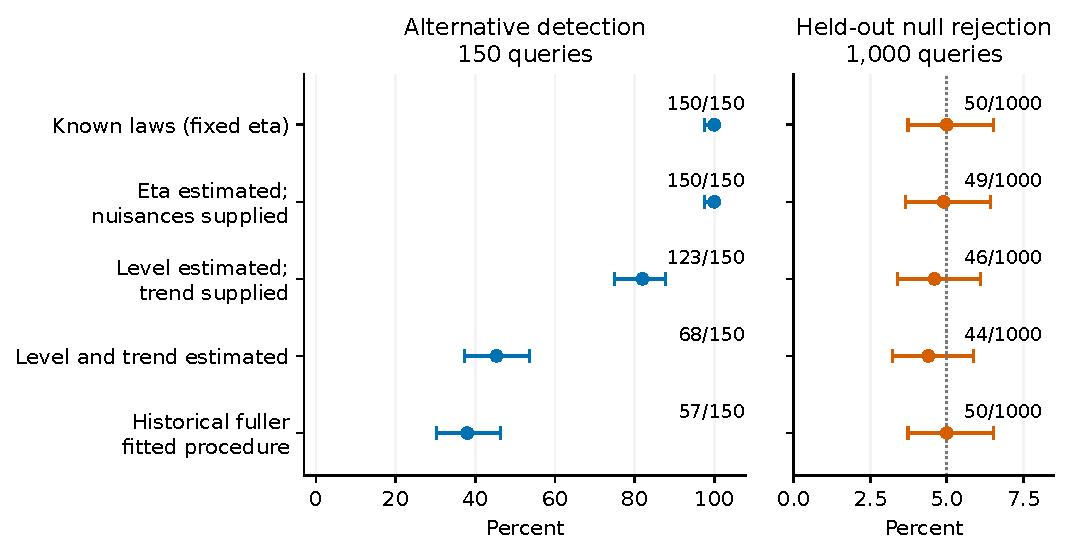
\includegraphics[width=\linewidth]{detection.pdf}
\caption{Historical matched-null detection on the same 150 stronger alternatives. Error bars are nominal conditional 95\% binomial intervals. Each procedure has its own 999 reference statistics and 1,000 separate null queries; adaptive selection and reference-bank uncertainty are omitted.}
\label{fig:detection}
\end{figure}

\section{Sensitivity to the diagnostic value}

The value of \(\eta\) changes the histories as well as the fixed-history intensity separation. In a paired comparison using the same \(150\) fresh pairs, the initial value \(\eta=0.2839974288868791\) produced \(49/150\) detections for the fuller fitted procedure, whereas the adjusted value \(\eta=0.4885010300470942\) produced \(57/150\). The paired gain is therefore \(8\) detected histories, or \(5.33\) percentage points, with a descriptive Monte Carlo standard error of \(4.71\) percentage points. A separate \(25\)-pair planning sample gave \(6/25\) and \(11/25\) under the two values; it is a planning exercise and is not pooled with the \(150\)-pair comparison.

The descriptive paired Monte Carlo standard error uses the sample variance of paired decision differences. For \(N_{\mathrm{pair}}\) pairs, let \(D_i\in\{-1,0,1\}\) be the first decision minus the second, with positive and negative discordance counts \(b,c\). Then
\[
 \overline D=\frac{b-c}{N_{\mathrm{pair}}},\qquad
 \widehat{\operatorname{MCSE}}
 =\sqrt{\frac{b+c-N_{\mathrm{pair}}\overline D^{\,2}}
 {N_{\mathrm{pair}}(N_{\mathrm{pair}}-1)}}.
\]
This is the sample standard deviation of \(D_i\) divided by \(\sqrt{N_{\mathrm{pair}}}\). Taking the adjusted-value decision first gives \(b=29,c=21\) and \(N_{\mathrm{pair}}=150\), hence \(4.7096\) percentage points, rounding to \(4.71\). Using empirical-variance divisor \(N_{\mathrm{pair}}\) instead gives a slightly different value from the same outcomes. The stated fixed-bank and adaptive-reuse qualifications still apply; no new test is added.

The mean achieved fixed-history total intensity suppression was \(14.159\%\) for the initial value and \(19.360\%\) for the adjusted value. For a realized nonempty history and fixed generating nuisance, the event-mean functional is
\begin{equation}
 S(\eta;\mathcal H_T)=\frac{100}{N_T}\sum_{i=1}^{N_T}
 \frac{B(t_i)\{1-e^{-\eta G_s(t_i)}\}}
      {B(t_i)+nH_e(t_i)}.
 \label{eq:achieved-suppression}
\end{equation}
Both intensities in each comparison use the same strictly earlier history. The reported mean then gives equal weight to each catalogue's event mean, rather than pooling every event across catalogues. This is the functional implemented in \hyperlink{S07}{archival \texttt{S07} (not distributed)}.
It is an event-mean description of separation on a common history, not a controlled reduction in earthquake count. Increasing \(\eta\) also changes the synthetic histories that are subsequently realized. Counts remain random, and no monotonicity of realized counts is guaranteed. An extreme retained pair, with \(449\) events under one member and \(6{,}553\) under the other, illustrates why suppression of a fixed-history rate cannot be reported as a promise about realized totals.

An earlier archive used a \(1{,}999\)-reference rank denominator of \(2{,}000\). The later recalibration using \(999\) references and \(1{,}000\) separate null queries produced the same count of \(57\) detections only by happenstance. It is a consistency observation, not an independent replication, and the two reference constructions should not be combined. The \href{https://github.com/Drefetr/InhibitoryEarthquakeModels/blob/3e76a174cf4f58ce601c6c9640c4d0c11168813f/paper/data/paired.json}{public paired summary} retains aggregate pairing results; the historical study is reported in \hyperlink{S08}{archival \texttt{S08} (not distributed)}. The completed-history provenance for later recalibration is recorded in \hyperlink{S09}{archival \texttt{S09} (not distributed)} and the final results in \hyperlink{S16}{archival \texttt{S16} (not distributed)}.

\section{Paired comparison of level and trend}

The level-and-trend comparison is more informative when the two procedures are paired on the same \(150\) histories rather than read only from marginal detection counts. Figure~\ref{fig:paired} crosses their decisions. Both procedures detect on \(62\) histories, the level-only procedure detects on \(61\) where the combined procedure does not, the combined procedure detects on \(6\) where level-only does not, and neither detects on \(21\). The marginal counts are therefore \(123\) and \(68\), and the difference is \(55/150=36.67\) percentage points, with a descriptive paired Monte Carlo standard error of \(4.58\) percentage points, using the same sample-variance convention with \(b=61,c=6\) and \(N_{\mathrm{pair}}=150\) (\(4.5776\) before rounding).

There is no pathwise dominance. The level-only procedure detects on \(61\) histories where the combined procedure does not, while the reverse occurs on \(6\). The \(55\)-history marginal gap is real for this realized paired bank, but the paired arrangement shows that it is not produced by a uniform improvement. Among the \(999\) null reference scores for the level-only procedure, \(604\) were exactly zero. Ties and the add-one rank rule are therefore material in that calibration. Different null thresholds can alter the comparison and must be considered when interpreting the paired decisions.

A ten-history raw-statistic pilot contained six null and four alternative histories. On that small pilot, level-only contraction exceeded trend-only contraction on four alternatives. This is a descriptive diagnostic of local score behavior, not a calibrated power comparison. That historical experiment does not contain a fully calibrated trend-only row, so the level-only discordance cannot be assigned uniquely to trend. The absence of that row does not imply that trend-only would perform best, nor does it automatically identify trend-only calibration as the best next experiment. A fair decision among procedures would require its own reference bank and calibration under the same reporting rules.

All \(1{,}150\) decisions in the reported historical detection-and-null evaluation resolved under the empirical numerical envelopes. That is a completeness statement for this realized study, not a rigorous universal bound on numerical integration or optimization. The selected-ten pilot is documented in \hyperlink{S15}{archival \texttt{S15} (not distributed)}. The paired detection table and matched-null results are documented in \hyperlink{S16}{archival \texttt{S16} (not distributed)}.


\begin{figure}[!htbp]
\centering
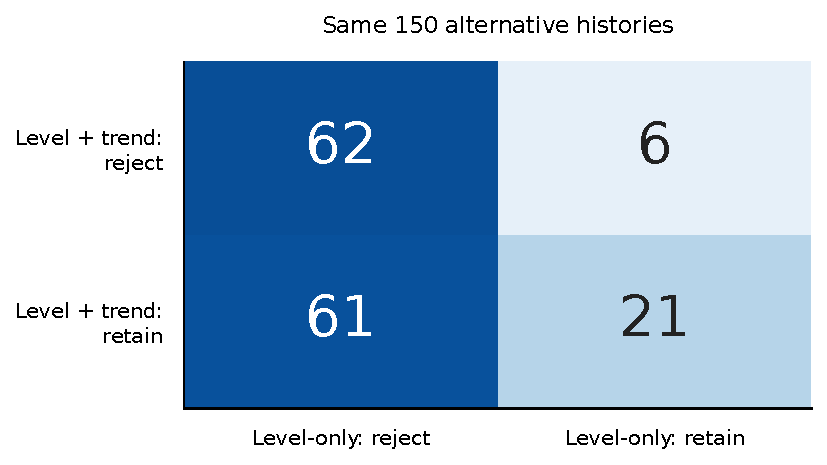
\includegraphics[width=0.68\linewidth]{paired.pdf}
\caption{Paired decisions for background level alone versus level and trend estimated. The 61 versus six discordant histories yield a 36.67 percentage-point net difference, but neither procedure dominates on every history.}
\label{fig:paired}
\end{figure}

\section{Diagnostics and limits of explanation}

A separate audit examined ten selected difficult completed histories using a larger iteration limit and a Powell search. The largest phase improvement in negative log likelihood was \(1.94995664\times10^{-8}\), and the largest direct generalized-likelihood-ratio change was \(3.89681745\times10^{-8}\), below the declared diagnostic screens of \(0.001\) for phase negative log likelihood and \(0.1\) for the direct statistic. These histories were selected because they were difficult, so the audit is neither representative of the full bank nor a global optimization guarantee. Within the audited set, however, it weakens an explanation of the fitted-law gap based on inadequate optimizer stopping. It does not eliminate the possibility of optimizer limitations on other histories. This selected-ten audit concerns the historical recipe; the later F solver diagnostics and unresolved outcomes are separately reported in the addendum.

Two pre-existing fixed-history score projections onto \(a\), \(d\), and \(n\) retain \(10.82\%\) and \(3.26\%\) of weighted \(\eta\) squared-score norms. These percentages show local overlap between the directions in which the background parameters and the diagnostic parameter move the score. They are not ensemble Fisher information, not fractions of statistical power, and not an explanation of the observed \(38\%\) fitted detection rate.

Saved likelihood accounting provides one further descriptive check: estimating background level and trend improved the selected null likelihood more than the alternative likelihood on all \(150\) histories, with median null negative-log-likelihood gain \(28.665\) versus \(0.862\) for the alternatives. This records how the supplied comparison accounted for background in these specific histories. It is not a measurement of physical loading. The optimizer audit is reported in \hyperlink{S14}{archival \texttt{S14} (not distributed)}; the score geometry is reported in \hyperlink{S02}{archival \texttt{S02} (not distributed)}; and the saved likelihood accounting is documented in \hyperlink{S11}{archival \texttt{S11} (not distributed)}.

Taken together, the matched studies locate a substantial change in calibrated detection when background parameters are estimated: under the stated synthetic law, the stronger alternatives are distinguishable with supplied laws and with \(\eta\) alone estimated, while fitting background components changes the calibrated detection outcome. The experiments cannot separate the unavoidable difficulty of a composite statistical problem from recoverable loss in a particular fitted procedure. They are controlled matched-law tests rather than empirical physical discovery, and the reported boundaries follow from that design. The scoped contribution is a reproducible, numerically explicit assessment of where the marked-sensitivity signal is retained or attenuated by estimation, together with the calibration limits needed to read it. 

The \href{https://github.com/Drefetr/InhibitoryEarthquakeModels/blob/3e76a174cf4f58ce601c6c9640c4d0c11168813f/paper/data/detection.json}{public detection summary} and the \hyperref[sec:source-supplements]{availability guide} provide public entry points. Saved summaries do not replace the omitted full authorities or historical history banks.

\section{A bounded four-procedure continuation}
\label{sec:f-continuation}

The accompanying \emph{F continuation: background nuisance estimation}
addendum (22 October 2026 revision; scientific execution on 19 October UTC)
reports a subsequent exploratory study. It uses the same pinned catalogue
and clock identities as the historical level-only and level-and-trend
studies, but fits a separately frozen finite numerical procedure with its
own mandatory solver and control rules. Every alternative estimates
\(\eta\); the background log level \(a\) and trend \(d\) are supplied or
estimated in a four-cell design. The supplied/supplied cell is therefore
distinct from the fixed-\(\eta\) known-law benchmark above.

\begin{table}[H]
\centering
\caption{Separate F continuation: decisions on all 150 planned alternative
queries at \(\alpha=0.05\). These counts belong to the new finite procedure,
not the historical table or its conditional binomial intervals.}
\label{tab:f-continuation}
\small
\begin{tabular}{@{}lrrr@{}}\toprule
Background nuisance fitted & Reject & Non-reject & Unknown\\\midrule
Neither (\(I_{00}\)) & 150 & 0 & 0\\
Level only (\(I_{10}\)) & 122 & 28 & 0\\
Trend only (\(I_{01}\)) & 150 & 0 & 0\\
Level and trend (\(I_{11}\)) & 65 & 82 & 3\\\bottomrule
\end{tabular}
\end{table}

All 2,149 identities remain registered, but only 7,068 of 8,596 planned
method outcomes have controlled statistics; 1,528 remain unknown. The
null-query rejection accounting bounds are \([0.030,0.407]\),
\([0.035,0.412]\), \([0.031,0.414]\) and \([0.031,0.411]\) in cell order,
using all 1,000 planned null queries. These are missing-decision bounds,
not confidence intervals. History cost, traversal and stopping rules make
missingness nonrandom. The continuation has not established its empirical
null size, and its alternative rejection fractions do not establish a
size-matched power ranking. Its full-pair interaction point mean and MCSE
remain unavailable. All 2,000 descriptive shared-reference/paired-query
resamples completed; their endpoint quantiles do not supply certified coverage.

A posthoc lineage check within the continuation fixed its original
25-query pilot cohort. The same level-only query fits and statistics gave
6 definite rejections, 11 non-rejections and 8 unknowns under the pilot
reference calibration, then 19, 6 and 0 under the expanded calibration.
This is calibration-dependent decision accounting. That 25-query cohort
is distinct from the earlier 25-pair \(\eta\)-planning sample reported
above. Neither comparison is an independent replication.

The trend-only cell now provides a bounded comparison under the new
procedure; it does not retrospectively explain the historical level-only
discordance. The addendum retains partial geometry diagnostics, failures,
methods and availability limits. The results support sensitivity to the
specified nuisance and calibration treatment, without identifying an
unavoidable loss, a physical mechanism or a universal benefit from a
particular nuisance restriction. The historical counts, intervals and
figures above remain results of their original recipes and are not pooled
with or overwritten by this continuation.


\chapter{Observed catalogue and held-out diagnostics}
\label{ch:observed}

\section{Scope and provenance of the archived catalogue}

The empirical analysis begins with an archived catalogue rather than with the unavailable inputs to the original manuscript. The primary archive is a GeoNet WFS snapshot downloaded on 15 October 2026. Events were selected with magnitude \(M\geq 5\) and depth no greater than \(40\)~km, within latitude \([-48.5,-33.5]\) and longitude \([165,180]\). The depth sentinel value \(-9\) was excluded, while other negative depths were retained. The resulting file contains 913 selected events in a 24,394-day observation window, from 1960-01-01 inclusive to 2026-10-15 exclusive. The event count is recorded, together with the filter definition and catalogue metadata, in the archived research report and processed metadata (\hyperlink{S25}{archival \texttt{S25} (not distributed)}; \href{https://github.com/Drefetr/InhibitoryEarthquakeModels/blob/3e76a174cf4f58ce601c6c9640c4d0c11168813f/provenance/catalogue_snapshot_metadata.json}{public metadata extract} (\texttt{S24})).

The reappearance of the number 913 does not establish identity with the event list analysed in the original work. The original frozen data, source configuration, and executable code are absent, so neither event identity nor processing history can be recovered. A second archived FDSN interface from the same provider returned 914 selections, consisting of 913 events common to the primary snapshot and the additional event 2025p672513. These are interface selections from one national provider, not independent physical catalogues. The interfaces share the same provider and much of their processing history; agreement between them cannot serve as independent validation of completeness or magnitude accuracy.

This distinction governs the interpretation of every later comparison. The reconstruction is an independent analysis applied to a documented archive snapshot, not a numerical replay of the historical analysis. The fitted catalogue slope for a continuous excess-exponential magnitude model is \(2.849401764894274\). For comparison with the earlier manuscript's half-bin convention, define
\[
 \widehat\beta_{\mathrm{adj}}
 =\frac{1}{\overline{M-M_0}+0.05},\qquad M_0=5.
\]
Applied to the archived selection, this gives \(2.494071218330174\), consistent in rounded form with the reported value near \(2.494\). This reconciles an estimator convention; mixed precision and native magnitude scales do not establish a common half-bin adjustment as a generally validated correction for this catalogue. The primary continuous estimate, raw magnitudes, productivity normalization and fitted-law records remain unchanged. It does not demonstrate that the historical event sample or likelihood calculation has been reproduced. Completeness above a time-varying threshold, the relation between native magnitude scales, missing parents of smaller or deeper events, activity before 1960, and the adequacy of national pooling therefore remain explicit assumptions (\hyperlink{S27}{archival \texttt{S27} (not distributed)}).


\begin{figure}[tbp]
\centering
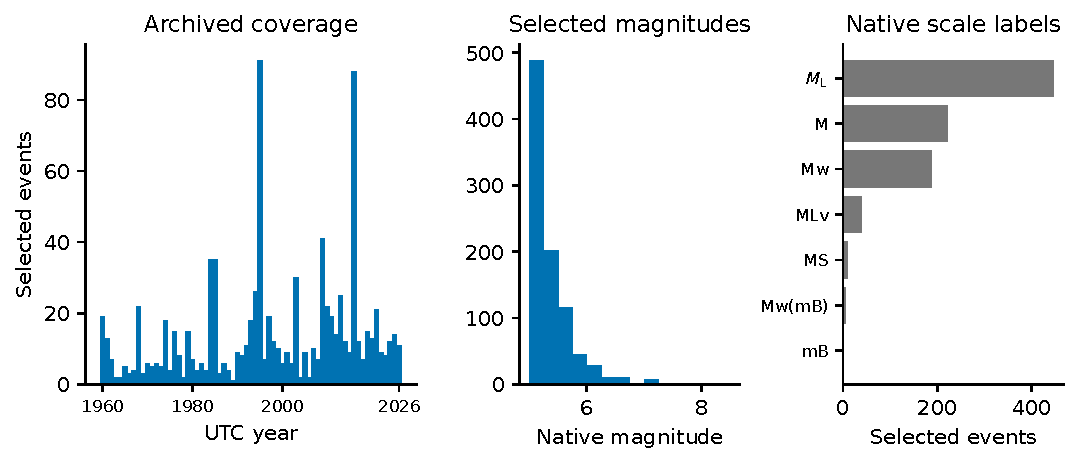
\includegraphics[width=\linewidth]{catalogue.pdf}
\caption{Descriptive summaries of the 913-event archived selection: annual counts, magnitudes and native magnitude labels. The final calendar year is partial. These plots describe this selection and do not establish catalogue completeness or homogeneous observation through time.}
\label{fig:catalogue}
\end{figure}

\section{A restricted diagnostic intensity}

The observed comparison uses the temporal diagnostic defined in the experimental design:
\begin{equation}
 \lambda_\eta(t)=B(t)e^{-\eta G_s(t)}+nH_e(t),\qquad
 B(t)=e^{a+d(2t/T_0-1)},\quad \eta\geq0.
 \label{eq:observed-diagnostic}
\end{equation}
Here the subscript \(s\) denotes stress memory and \(e\) denotes excitation. Neither denotes a spatial coordinate. Both features depend only on strictly earlier events. The implemented Mittag--Leffler (ML) kernels are finite positive spectral mixtures. A shared-memory recipe supplies the same kernel parameters to the stress and triggering features, although those features enter different parts of the intensity. The background is specified independently of the stress history. Thus this family diagnoses a restricted form of inhibition; it does not reproduce the original physical loading construction.

The five observed candidate families were constant Poisson, loglinear Poisson, Omori triggering, ML triggering, and ML triggering with shared inhibition. The principal contrasts compare the last three families. Model labels use ``ML'' for Mittag--Leffler. The native local-magnitude label in Figure~\ref{fig:catalogue} is displayed as \(M_{\mathrm L}\); the original archive label is retained in the data. All five families and their search rules are recorded in \href{https://github.com/Drefetr/InhibitoryEarthquakeModels/blob/3e76a174cf4f58ce601c6c9640c4d0c11168813f/engine/iteration_27/configs/observed_frozen.json}{public search protocol (operational adaptation)} (\texttt{S18}).

The temporal Omori comparator uses the normalized triggering density
\[
 h_{\mathrm O}(u;c,p)=\frac{p-1}{c}\left(1+\frac{u}{c}\right)^{-p}
 =(p-1)c^{p-1}(u+c)^{-p},
 \qquad u\geq0,\quad c>0,\quad p>1.
\]
The lag \(u\) is measured in days. Its integral on $[0,\infty)$ is one. The scale $c$ is measured in days and
is stored as \texttt{KernelSpec.tau}; the triggering multiplier $n$ remains
separate. This specifies the temporal comparator used here, not a complete
space--time ETAS construction.

The split is chronological. The absolute trend coordinate is \(x=2t/T_0-1\), where \(T_0=24394\) days. Candidate fits use the first \(0.50\), \(0.65\), and \(0.80\) fractions of the archive horizon as training prefixes, comprising 301, 504, and 659 events. Tests use the following disjoint intervals \(0.50\)--\(0.65\), \(0.65\)--\(0.80\), and \(0.80\)--\(1.00\), containing 203, 155, and 254 events and 612 test events in total. These intervals correspond approximately to 1993--2003, 2003--2013, and 2013--2026, but the fractions and archive day indices are the operative definitions.

All retained history before each origin, including earlier test history, is available to the candidate intensity. Each fit uses only its training prefix. The exponential mark-rate estimate is obtained from training marks alone and is common across candidate families; it is a plug-in estimate rather than a joint marked-intensity maximum-likelihood estimate. The reported score is the full marked-event score: the sum of event log intensities and log mark densities minus the integrated intensity over quiet exposure, with the final censor handled explicitly in the declared protocol. The uninhibited fit is retained as an exact eligible point in the inhibited search, so nonnegative training gain is partly built into candidate selection. This fact limits any inference from training improvement alone. The stored training gains for the shared diagnostic are \(2.731009\), \(0.302486\), and \(0.143866\), but those numbers are not treated as evidence of predictive success.

\subsection{Saved parameters at the predictive origins}\label{sec:saved-fits}
Table~\ref{tab:saved-predictive-parameters} displays the saved selected records for the three triggering families at the three predictive origins, not new fits. The \href{https://github.com/Drefetr/InhibitoryEarthquakeModels/blob/3e76a174cf4f58ce601c6c9640c4d0c11168813f/paper/supplements/predictive_parameters.json}{selected-parameter companion}
% Exact companion path: supplements/predictive_parameters.json
 retains all fifteen records for the five families, full precision, source hashes and field pointers. The constant Poisson model fixes \(d=n=\eta=0\); loglinear Poisson fixes \(n=\eta=0\). The table's two uninhibited triggering families fix \(\eta=0\).

\begin{table}[htbp]
\centering\small
\setlength{\tabcolsep}{4pt}
\caption{Saved selected parameters at three predictive origins. The background is \(\exp(a+dz(t)-\eta G_s(t))\) per day, with \(z(t)=2t/24394-1\). Values are rounded for display; zeros in the uninhibited families are fixed.}
\label{tab:saved-predictive-parameters}
\begin{tabular}{llrrrr}
\toprule Origin & Family & \(a\) & \(d\) & \(n\) & \(\eta\) \\ \midrule
50\% & Omori & $-4.712517$ & $-0.457071$ & 0.685640 & 0.000000 \\
50\% & Mittag--Leffler & $-4.458572$ & $-0.252150$ & 0.455824 & 0.000000 \\
50\% & Shared inhibition & $-2.196743$ & 1.789757 & 0.481700 & 1.646714 \\
65\% & Omori & $-4.291554$ & 0.048036 & 0.570076 & 0.000000 \\
65\% & Mittag--Leffler & $-4.188810$ & 0.147441 & 0.497996 & 0.000000 \\
65\% & Shared inhibition & $-3.841844$ & 0.492682 & 0.503490 & 0.211710 \\
80\% & Omori & $-4.394252$ & $-0.196162$ & 0.561216 & 0.000000 \\
80\% & Mittag--Leffler & $-4.282575$ & $-0.056651$ & 0.470292 & 0.000000 \\
80\% & Shared inhibition & $-4.103408$ & 0.127638 & 0.473071 & 0.105254 \\
\bottomrule
\end{tabular}
\par\medskip
\begin{tabular}{lrrrr}
\toprule Origin & \(\beta_{\rm train}\) & \(r\) & Omori \(c\) (days) & Omori \(p\) \\ \midrule
50\% & 3.101622 & 0.4 & 0.012995 & 1.113368 \\
65\% & 3.149488 & 0.7 & 0.020798 & 1.198604 \\
80\% & 3.021907 & 0.7 & 0.006972 & 1.155845 \\
\bottomrule
\end{tabular}
\end{table}

All six selected Mittag--Leffler kernels use \(\alpha=0.5\), the lower searched grid endpoint, and \(\tau=1\) day, an interior grid value. The common selected productivity ratio is \(r=0.4\) at the first origin and \(r=0.7\) at the later origins; the former is the lower searched ratio endpoint. The Omori coordinates \(c,p\) were optimized continuously with a retained coarse-grid floor; they are not merely grid winners. These endpoint descriptions are newly checked arithmetic against the frozen search grids. Historical boundary flags, tolerance-based near-boundary classifications and standard errors were not saved. The selected continuous coordinates are strictly inside their recorded bounds under exact comparison. No uncertainty estimates are inferred.

The rates \(\beta_{\rm train}\) are estimated from training marks alone, held common across families, and frozen during each test. Inactive serialization fields are not fitted coordinates: the saved \(p\) field of a Mittag--Leffler kernel and \(\alpha\) field of an Omori kernel have no role in their respective formulas. 

At the three predictive origins, the selected shared-inhibition recipe's
unattenuated deterministic background is approximately \(9.60\), \(1.57\)
and \(1.34\) times that of the corresponding noninhibited Mittag--Leffler
recipe, respectively. The first-origin fit therefore combines a much larger
baseline with stronger depletion. These are descriptive ratios of fitted
components, not total-intensity ratios or a demonstrated causal explanation
of the subsequent predictive loss.

\section{Earlier calibrated restrictions}

The earlier reconstructed analysis tested two restrictions: no feedback and a common rather than separate memory scale. Its observed statistics were \(0.7036472\) and \(0.0829952\), respectively. The completed fitted-law calibration retained \(1{,}999\) null cases per restriction, giving add-one ranks of \(0.365\) and \(0.263\). Neither restriction was rejected by that declared five-percent procedure. These are conditional ranks, not probabilities that the hypotheses are true. In particular, non-rejection does not demonstrate equal physical memories, and the stress kernel's disappearance at zero feedback limits what such a restriction can establish. The calibration authority is \hyperlink{S01}{archival \texttt{S01} (not distributed)}; its interpretation is summarized in \hyperlink{S27}{archival \texttt{S27} (not distributed)}.

The later chronological comparison asks a different question: do the declared inhibited recipes predict subsequent observations better than serious triggering alternatives? A negative predictive result need not contradict a non-rejecting in-sample restriction test. Their targets, fitting rules and calibration differ.

\section{Held-out score comparison}

Table~\ref{tab:observed-scores} reports score differences relative to the ML triggering-only benchmark. Negative values favour the benchmark; positive values favour the named alternative.

\begin{table}[!ht]
\centering
\caption{Held-out marked-process score differences relative to the ML triggering-only benchmark. Tests are disjoint chronological intervals in the declared archive protocol. Values are differences, not log-likelihoods for separate datasets.}
\label{tab:observed-scores}
\small
\setlength{\tabcolsep}{4pt}
\begin{tabular}{lrrrr}
\toprule
Contrast & Test 1 & Test 2 & Test 3 & Total \\
\midrule
Shared inhibition \(-\) ML & \(-16.517557\) & \(-0.075277\) & \(-1.030025\) & \(-17.622859\) \\
Omori triggering-only \(-\) ML & \(+3.106623\) & \(+2.837708\) & \(+6.513790\) & \(+12.458121\) \\
\bottomrule
\end{tabular}
\end{table}

The shared diagnostic loses in all three folds. Its total disadvantage is driven overwhelmingly by the first block: approximately \(93.7\%\) of the total deficit occurs there. The second-block difference is nearly zero, but that is not strong independent evidence of parity because the training histories overlap and later folding choices were inspected during development. The calculations are exploratory and were not designed as confirmatory or as an independent sequence of repeated tests (\hyperlink{S19}{archival \texttt{S19} (not distributed)}).

The continuous Omori recipe improves on the finite ML kernel grid in every fold. This result cannot be converted into a universal law ranking. The Omori refinement and the finite spectral ML candidate have unequal flexibility, and the contrast therefore favours the declared Omori recipe under its fitting convention. It is not an isolated estimate of the effect of \(\eta\), nor a demonstration that every continuously refined triggering model dominates every grid-based alternative. Residual diagnostics were descriptive, varied over the record, and did not certify any winner as an adequate physical model.


\begin{figure}[tbp]
\centering
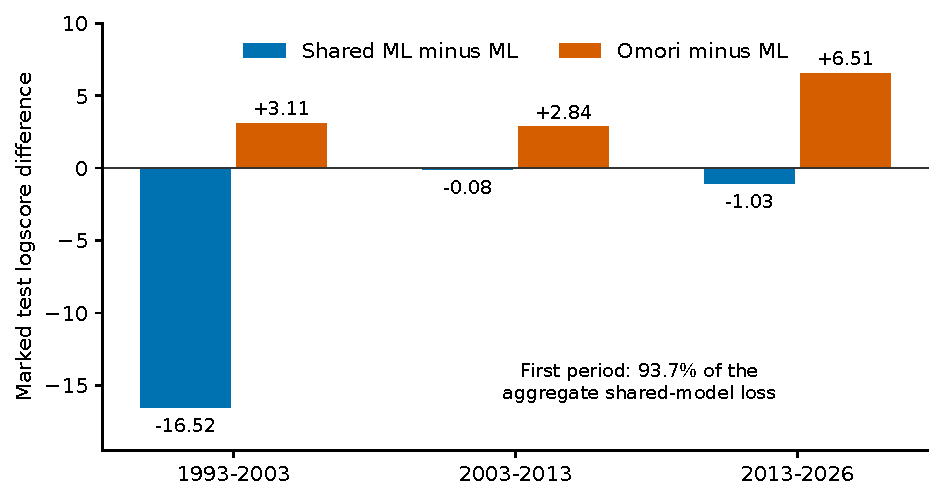
\includegraphics[width=\linewidth]{prediction.pdf}
\caption{Chronological test-score contrasts for the declared recipes. The first test block contributes about 93.7\% of the aggregate shared-inhibition disadvantage. Training prefixes overlap and the periods were reused in exploratory development; the three periods are not independent confirmatory tests.}
\label{fig:prediction}
\end{figure}

\section{Score accounting and temporal localization}

For a fold, write the score difference as
\begin{equation}
  \Delta\ell
  = E+C,
  \qquad
  E=\sum_i\log\frac{\lambda_{\mathrm{sh},i}}{\lambda_{\mathrm{ML},i}},
  \qquad
  C=\Lambda_{\mathrm{ML}}-\Lambda_{\mathrm{sh}},
  \label{eq:score-accounting}
\end{equation}
where the event sum uses pre-event intensities at the realized times, and \(\Lambda\) denotes the corresponding integrated intensity. This separates event-term disagreement from realized compensator disagreement. In the first test block,
\[
E=-33.715205,\qquad C=17.197647,\qquad \Delta\ell=-16.517557.
\]
The integrated intensities are \(115.871595\) under the shared diagnostic and \(133.069242\) under the ML benchmark for 203 events. These are not conventional expected counts from a fixed fitted Poisson model: the compensator is evaluated along an updating estimated history. Its realized value is not automatically the future expected count conditional only on information at the test origin. No naive Poisson count probability value is attached to their difference.

Four equal-duration bins within the first test interval sharpen the accounting without allocating events to bins by any counterfactual rule. Each bin uses the complete preceding history and integrates over its own realized path. Approximate calendar labels are displayed only for orientation; the archive-day boundaries define the calculation.

\begin{table}[!ht]
\centering
\caption{Score accounting within four equal-duration subintervals of the first test block. Each row uses full preceding history and realized integration within that subinterval.}
\label{tab:first-block-accounting}
\small
\setlength{\tabcolsep}{4pt}
\begin{tabular}{lrrr}
\toprule
Approximate interval & \(E\) & \(C\) & \(\Delta\ell\) \\
\midrule
1993-05-24 to 1995-11-24 & \(-2.891244\) & \(2.464270\) & \(-0.426975\) \\
1995-11-24 to 1998-05-27 & \(-16.875378\) & \(7.143815\) & \(-9.731563\) \\
1998-05-27 to 2000-11-27 & \(-8.696131\) & \(4.642115\) & \(-4.054016\) \\
2000-11-27 to 2003-05-31 & \(-5.252451\) & \(2.947447\) & \(-2.305004\) \\
\bottomrule
\end{tabular}
\end{table}

The deficit is localized in time rather than uniformly spread across the first block. The strongest subinterval loss occurs between approximately late 1995 and mid-1998. This localization does not identify an earthquake sequence, a geological province, or a causal mechanism. It records that the aggregate score is sensitive to when an updating history and its compensator disagree (\hyperlink{S20}{archival \texttt{S20} (not distributed)}).


\begin{figure}[tbp]
\centering
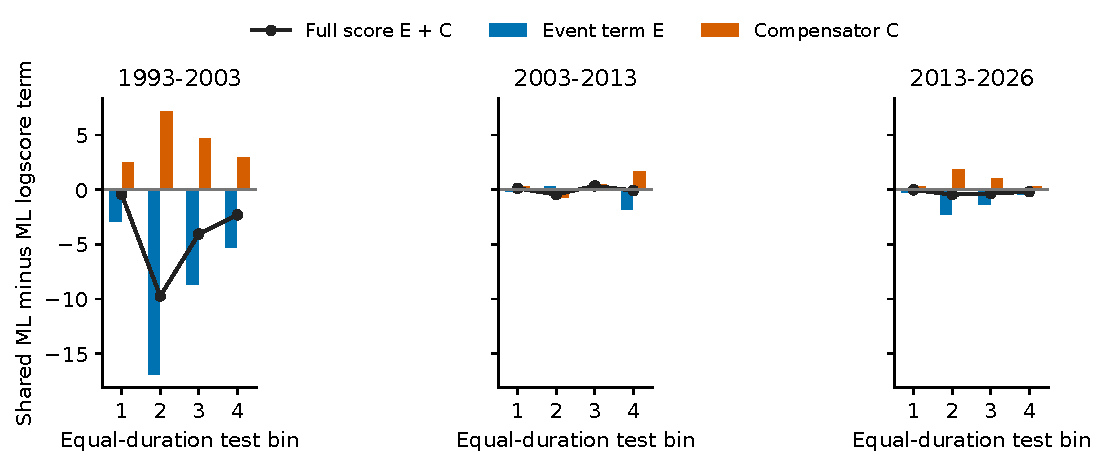
\includegraphics[width=\linewidth]{temporal.pdf}
\caption{Event and compensator contributions in four equal-duration bins in each of the three test periods. Each bin is integrated with complete preceding history. In the first period a favorable compensator contribution partly offsets the negative event term; the full score is their sum.}
\label{fig:temporal}
\end{figure}

A spatial and mark audit found that all five occupied coarse cells had negative event-term contributions for the shared-minus-benchmark contrast. The same direction appeared for native ML and \(M_{\mathrm w}\) magnitude conventions and for all declared magnitude and depth groups. The shared specification contains one regional compensator rather than cell-specific or group-specific exposure. Accordingly, these sums are diagnostics of event-term sign under the fitted family, not local likelihoods, local rates, or fractions of the full score. Unequal cell areas, time-location confounding, sparse cells, and reuse of events across overlapping marginal classifications prevent such a local interpretation. Grouping by the current event's mark is descriptive: that mark affects subsequent intensity and does not enter its own pre-event intensity. Native magnitude-label composition changes most strongly in the last block, whereas the dominant loss is in the first, weakening a simple explanation based only on a modern label transition. Completeness and legacy magnitude-scale concerns remain.

\section{Archive sensitivity and a bounded horizon check}

A replacement audit matched all 913 event identifiers and found 241 numerical magnitude differences, the largest absolute difference being \(0.164143665\). Many differences were only in small decimal places. The full history was rescored using alternate matched magnitudes while primary clocks, locations, depths, the fitted \(\beta\), and the recipe definitions were fixed. The additional event in the 914-event interface selection was excluded, and no parameters were refitted or physically converted between magnitude scales.

Under this replacement, the total shared score changed as follows:
\[
 -17.622859365\ \longrightarrow\ -17.617975447,
 \qquad \text{change }+0.004883918.
\]
No fold changed sign. The Omori total changed from \(12.458121\) to \(12.441651\), shown to six decimal places. Thus the tested archive value discrepancy does not explain the recipe failure. Equally, this bounded audit does not eliminate every observational uncertainty in magnitudes, depths, locations, completeness, or event identity.

A separate horizon-feasibility pilot was restricted and incomplete: 27 of 30 declared horizon-prefix cases completed, one was resource-limited, and two remained pending. Five null paths at a given horizon cannot calibrate a five-percent add-one test: the smallest possible rank is \(1/6\). This is neither a power calculation nor a certificate of sufficient sample size. No incomplete case is treated as a non-rejection, and no resumed or future campaign is claimed. The pilot concerns restricted fitting feasibility. It supplies no calibrated detection decisions or minimum-event requirement.

The observed evidence in this chapter is therefore selective and conditional. The held-out scores are unfavourable to the implemented shared-inhibition recipes, the source-magnitude audit does not reverse that pattern, and the strongest loss is temporally localized. These findings constrain the current diagnostic families. They do not establish the absence of physical shared memory in the Earth system.

The \href{https://github.com/Drefetr/InhibitoryEarthquakeModels/blob/3e76a174cf4f58ce601c6c9640c4d0c11168813f/paper/data/prediction.json}{public predictive summary} and the \hyperref[sec:source-supplements]{availability guide} provide public entry points. Saved summaries do not replace the omitted full authorities or historical history banks.

\chapter{Discussion and limits of inference}
\label{ch:discussion}

\section{What the theory separates}

The mathematical results delimit several distinct regimes. Finite positive-mode systems admit the stated first-moment stability conclusions under their link, mark and subcritical-triggering assumptions. Finite-horizon approximation does not establish an interchange of stationary and infinite-mode limits. Exact-memory counterexamples apply to specified no-feedback submodels, and the linear-response calculation concerns an auxiliary frozen-slope system. Full-law identifiability also requires assumptions stronger than those available in an observed finite catalogue. The preceding mathematical chapters state their assumptions and proofs.

This separation matters for the empirical discussion. A physical model may contain loading or initial-stress memory while a finite catalogue lacks power to distinguish it from a restricted alternative. A diagnostic family may improve its training score because its likelihood geometry favours extra structure, without thereby identifying the full physical law. A small held-out loss may be numerically controlled yet limited as statistical evidence when folds overlap or were inspected. Conversely, a non-rejection is not evidence of equality. Failure to distinguish two recipes leaves a set of explanations: the data may be insufficient, the candidate may be misspecified, the optimizer may be imperfect, or the tested effect may be small over the observed horizon. The controlled studies weaken some specific explanations, but do not select a unique physical one.

At \(\eta=0\), a separately varied stress kernel disappears from the diagnostic intensity when background and triggering are held fixed. It is therefore unidentified there. The analogous physical loading argument requires finite loading and initial-stress parameters: it cannot be carried into a singular small-feedback, large-loading limit without additional analysis. Non-rejection of a shared-kernel restriction at or near zero feedback consequently does not validate equality of two physical memories.

Synthetic diagnostics further clarify, but do not erase, the inferential gap. The historical comparison with nuisance quantities supplied produced 150 detections in 150 trials, whereas a fitted setting produced 57 in 150. These are different simple-versus-composite inferential tasks; their contrast is not an intrinsic information ceiling, and it is not proof that the remainder is avoidable algorithmic inefficiency. It offers no justification for fixing the real background merely to recover apparent power. Better optimization or a larger synthetic bank can improve numerical precision without changing the scientific question. The later F continuation (Section~\ref{sec:f-continuation}) adds a trend-only cell under a different finite procedure and demonstrates calibration-dependent decisions on unchanged pilot fits. Its incomplete null coverage prevents an established size-matched power comparison; it supplies no causal explanation for the historical fitted-law gap.

The transformed marks add another qualification. The magnitude excess has an exponential law, while the stress and productivity transforms have finite first and infinite second moments at the declared generating parameters. That does not prevent bounded-indicator Monte Carlo summaries, but it invalidates unqualified use of Fisher-information shortcuts based on second moments. Computational stability and statistical efficiency therefore have to be defended under the declared scoring rule, not inferred from formal differentiability alone.

\section{What regional nonclosure means}

Proposition~\ref{prop:regional_nonclosure} and Figure~\ref{fig:pooling} give a precise reason to examine the scale of aggregation. Summing locally inhibited background contributions generally differs from inhibiting a summed national history. Two regional configurations can have the same total depletion but different aggregate local intensities; one national coefficient cannot restore information already discarded by summation. The effective depletion depends nonlinearly on regional history and background shares.

This is conditional algebra, not evidence that pooling caused the observed predictive failure. Restricted regional configurations can admit closure, while the aggregation of triggering and the conditioning on unobserved regional labels introduce further questions. The catalogue audit has not fitted a spatial conditional intensity or measured a geological stress-transfer mechanism. Its event-only maps motivate an adequacy question without answering it.

\section{An explicitly optional locality extension}

One possible extension would compare, on the same region-labelled observations, three deliberately matched candidates: no inhibition, pooled inhibition across regions, and local inhibition. For a given regional history, schematic intensities could be written as
\begin{align}
  \lambda_k^{(0)}&=B_k+H_k, \label{eq:locality-none}\\
  \lambda_k^{(\mathrm{pool})}
    &=B_k\exp\!\left(-\eta\sum_jG_j\right)+H_k, \label{eq:locality-pooled}\\
  \lambda_k^{(\mathrm{local})}
    &=B_k\exp(-\eta G_k)+H_k, \label{eq:locality-local}
\end{align}
where \(H_k\) includes the trigger amplitude and must be defined identically across alternatives. A fair comparison would match spatial backgrounds, triggering families with a serious Omori baseline, mark and history rules, observation rules, and fitting effort. With region label \(r_i\) for event \(i\), every candidate would use the same joint score
\begin{equation}
 \ell=\sum_i\log\lambda_{r_i}(t_i-)
      -\sum_k\int_0^T\lambda_k(t)\,\dif t
      +\sum_i\log f(m_i).
 \label{eq:proposed-spatial-score}
\end{equation}
The integrals include quiet regions and quiet intervals. Omitting them would reward or penalize models according to event allocation without accounting for exposure. Alternatively, all candidates would have to be marginalized to the same label-discarded observations; a label-aware likelihood and a label-discarded likelihood cannot be ranked as if they used the same data event.

This is a proposed extension rather than a completed experiment. The present conclusions do not depend on its outcome. Any future region and training choices would need to be declared before new test outcomes, avoiding selection on the losses already observed. Nor is there a promise that local formulation would recover a physical mechanism.

\section{Contribution and limits}

Taken together, the work makes a connected contribution in three parts. First, restricted mathematics establishes first-moment results for finite-mode systems and separates those results from unresolved nonlinear infinite-memory questions. Second, finite-history likelihood calculations and null-calibration controls show that detection is background sensitive and that a numerical score advantage must be separated from sampling calibration. Third, the archived observed exercise supplies held-out score evidence unfavourable to the current inhibited recipes, while source and temporal sensitivities narrow the explanations available for that failure.

These conclusions are bounded by the catalogue and designs that produced them. The observed catalogue is finite; its completeness, magnitude-scale compatibility, missing parents, and spatial limits remain assumptions. Candidate models are restricted, the selected periods were reused adaptively, and null-bank uncertainty remains. The fitted optimum is not certified globally, and the distinction between finite and infinite memory cannot be settled by a finite sequence alone. Priority remains unresolved for the component results identified in Appendix~\ref{app:literature_status}; the classifications there make no firstness claim.

More Monte Carlo runs under the same procedure can improve precision, and more events may improve some finite-catalogue summaries, but neither supplies a universal guarantee of detection or identification. The manuscript therefore closes on supported claims rather than a forced positive discovery: the implemented observed held-out comparisons do not support the current shared-inhibition recipes as predictive successes; non-rejection elsewhere does not prove equality; and the theoretical and algebraic results delimit what may and may not be concluded from those facts.

\chapter{Conclusion}
\label{ch:conclusion}

The mathematical legitimacy of an inhibitory point process, identification of its observation law and predictive value of a fitted recipe are separate achievements. The present contribution connects them through restricted stability and identification results, controlled nuisance-sensitivity comparisons and exploratory prediction in a reconstructed earthquake catalogue.

The finite-mode physical model supports first-moment stability under explicit sign, mark, state-domain and coupling assumptions. Infinite stationary second moments can coexist with that result. Finite-horizon approximation does not exchange infinite-mode and stationary limits, and the no-feedback exact-memory counterexamples establish an obstruction without settling active nonlinear inhibition. At zero feedback the diagnostic stress kernel disappears from the observation law. Positive-feedback identification is possible under the stated full-law assumptions, including known transforms and rich mark support; it is not a guarantee of stable finite-catalogue estimation. Conditional amplitude profiling and fixed-rule score response provide further finite-history tools within those boundaries.

The controlled experiments change the interpretation of weak fitted detection. The known-law procedure detected 150/150 saved alternatives, with 50/1,000 separate null rejections. Background level estimation retained 123/150 detections when trend was supplied; estimating level and trend retained 68/150. These are pronounced procedure differences under the declared law. The oracle receives additional nuisance information, so the contrast does not separate unavoidable composite-testing difficulty from recoverable procedure inefficiency. Fixing unknown real-data backgrounds merely to reproduce the synthetic advantage would be unjustified.

In the observed comparison, the shared-inhibition recipe improved score in none of three declared periods, while an Omori triggering comparator scored better than Mittag--Leffler triggering. Approximately 93.7\% of the inhibition recipe's aggregate disadvantage occurred in the first period; one later contrast was almost zero. Reused periods, overlapping training prefixes, unequal kernel flexibility and residual adequacy concerns restrict the result to exploratory recipe comparisons. It is useful negative predictive evidence, without establishing the presence or absence of physical inhibition or shared material memory.

The aggregation calculation gives a substantive reason to investigate locality: equal pooled depletion can conceal different aggregate local rates. A bounded comparison of no inhibition, pooled inhibition and local inhibition would need common observations, matched backgrounds, serious triggering benchmarks and complete regional compensators. This remains an extension rather than a condition for the existing contribution. The next empirical question is whether locality adds predictive information after background and triggering structure have been matched, rather than whether another search can produce a preferred sign.

\appendix
\chapter{Evidence and reproducibility}
\label{app:evidence}

\section{What the manuscript and its companion files reproduce}

The companion source builds this manuscript and its figures from explicit equations and saved numerical summaries. It does not rerun the historical scientific studies. Rebuilding a plot from a retained table is different from regenerating its histories, refitting its models and recalibrating its test. Each derived data file and figure records its source in the figure manifest. Illustrative mathematical figures are labelled as such; they are not synthetic catalogue outcomes.

The earlier 40-page manuscript and third-party catalogue records are not redistributed in this public repository. The catalogue provider, access locations, selection rules, original snapshot hashes and terms are documented in \path{docs/data.md}. Reacquiring a live catalogue does not guarantee recovery of the historical snapshot. The earlier manuscript's frozen catalogue, original fitting code, complete optimization records and editable source remain unavailable.

The principal data snapshot was retrieved on 15 October 2026 from GeoNet's WFS interface. Its selected CSV is \path{iteration_5/data/processed/geonet_M5_shallow_1960_2026.csv}, with SHA256
\begin{quote}\small\ttfamily
feacccb7581d1c4c33f88874cd6b198c41639da6930a7fc35e46f910a594fb3e.
\end{quote}
The saved metadata defines the exact geographic, depth, magnitude, event-type and clock rules. The 1960-origin observation window is 24,394 days, with 15 October 2026 excluded. The archived FDSN selection contains 914 events: all 913 primary IDs and one additional ID. These are two interfaces/snapshots from one provider, not independent physical catalogues.

\section{Canonical authorities for the main results}

Table~\ref{tab:authority_map} gives the archive-relative entry points needed to inspect the main claims. Narrative summaries point to their underlying machine-readable outputs. A source report establishes what was reported and retained; a hash establishes byte consistency. Neither alone certifies a physical mechanism or every historical execution.

The public per-authority register \path{paper/supplements/source_availability.json} records which files are included here and which remain references to the research archive. The historical source index is retained as metadata in \path{provenance/historical_v4_source_index.json}; its old included paths describe release v4, not this repository. The compact public repository retains the reusable numerical implementation and selected result summaries, rather than the complete investigation record. No third-party event records or earlier manuscript PDF are redistributed.

\begin{longtable}{@{}>{\raggedright\arraybackslash}p{0.20\textwidth}>{\raggedright\arraybackslash}p{\dimexpr\textwidth-0.20\textwidth-2\tabcolsep\relax}@{}}
\caption{Canonical source map. Display names identify archive-relative authorities; stable IDs map to the full paths in the source index. This is not a promise that every historical payload is embedded in a compact manuscript release.}\label{tab:authority_map}\\
\toprule
Topic & Authority and scope \\
\midrule
\endfirsthead
\toprule Topic & Authority and scope \\\midrule
\endhead
Finite-mode analysis & \nolinkurl{A_finite_mode_audit.md}; accompanying \texttt{S21}: \nolinkurl{A_theorems.tex}. State assumptions, construction, coupling and approximation scope. \\
% Exact archive paths: iteration_4/reports/A_finite_mode_audit.md; iteration_4/manuscript_revisions/A_theorems.tex
Exact memory and response & \nolinkurl{B_memory_response.md}; \texttt{S22}: \nolinkurl{B_propositions.tex}. No-feedback obstructions and the auxiliary response are separate results. \\
% Exact archive paths: iteration_4/reports/B_memory_response.md; iteration_4/manuscript_revisions/B_propositions.tex
Identification and score bounds & \texttt{S23}: \nolinkurl{C_identifiability.md}; \texttt{S03}: \nolinkurl{restricted_score_bound.md}; \texttt{S06}: \nolinkurl{power_response_corollary.md}. Positive-feedback and fixed-rule assumptions apply locally to each proposition. \\
% Exact archive paths: iteration_4/reports/C_identifiability.md; iteration_13/reports/restricted_score_bound.md; iteration_15/reports/power_response_corollary.md
Amplitude profiling & \texttt{S12}: \nolinkurl{A_amplitude_proposition.md}; \texttt{S13}: \nolinkurl{background_balance_corollary.md}. Conditional negative-log-likelihood calculus, not a global optimizer theorem. \\
% Exact archive paths: iteration_23/reports/A_amplitude_proposition.md; iteration_23/reports/background_balance_corollary.md
Reconstructed catalogue & \texttt{S24}: \nolinkurl{catalogue_metadata.json}; \texttt{S25}: \nolinkurl{research_report.md}. Archived new snapshot, selection and independent reconstruction. \\
% Exact archive paths: iteration_5/data/processed/catalogue_metadata.json; iteration_5/reports/research_report.md
Known-law comparison & \texttt{S09}: \nolinkurl{completed_evaluation.md}; \nolinkurl{completed_results.json}. All 2,149 scores accepted, including five validated imports; no new histories for this comparison. \\
% Exact archive paths: iteration_19/reports/completed_evaluation.md; iteration_19/reports/completed_results.json
Background comparison & \texttt{S11}: \nolinkurl{research_report.md}; \nolinkurl{completion_summary.json}. Accepted completion of the supplied-background and estimated-background procedures. \\
% Exact archive paths: iteration_22/reports/research_report.md; iteration_22/results/completion_summary.json
Optimizer robustness & \texttt{S14}: \nolinkurl{research_report.md}. Ten selected difficult histories; the earlier preparation and failed strict branches are not substituted for completion. \\
% Exact archive paths: iteration_24/completion/reports/research_report.md
Raw ablation & \texttt{S15}: \nolinkurl{research_report.md}. Ten-history level/trend raw-statistic comparison, not calibrated power. \\
% Exact archive paths: iteration_25/completion/reports/research_report.md
Level-only calibration & \texttt{S16}: \nolinkurl{research_report.md}; \texttt{M09}: \nolinkurl{summary.json}. All 2,149 fresh fits and accepted matched-null decisions. \\
% Exact archive paths: iteration_26/completion/reports/research_report.md; iteration_26/completion/results/summary.json
Observed prediction & \texttt{S19}: \nolinkurl{research_report.md}; \texttt{M18}: \nolinkurl{summary.json}. Three folds, five declared families, 612 scored test events. \\
% Exact archive paths: iteration_27/reports/research_report.md; iteration_27/results/observed_analysis/summary.json
Heterogeneity and source sensitivity & \texttt{S20}: \nolinkurl{research_report.md}; \nolinkurl{summary.json}; \nolinkurl{A_source_comparison.json}. Fixed-parameter temporal decomposition and matched source-value sensitivity. \\
% Exact archive paths: iteration_28/reports/research_report.md; iteration_28/results/publication/summary.json; iteration_28/results/A_source_comparison.json
\bottomrule
\end{longtable}


\section{Stable source supplement identifiers}\label{sec:source-supplements}
The identifiers below replace internal report-title fragments in the main text. Each points to the exact archived document, not to a proposition in this manuscript. The public repository retains their stable identifiers and historical paths as provenance metadata; the public availability register identifies the subset actually included. Historical documentary reports are not all distributed here. These are documentary sources, not newly reproduced scientific runs.
% Exact archive paths: supplements/source_evidence/; supplements/source_index.json

\begin{longtable}{@{}>{\raggedright\arraybackslash}p{0.09\textwidth}>{\raggedright\arraybackslash}p{\dimexpr\textwidth-0.09\textwidth-2\tabcolsep\relax}@{}}
\caption{Stable documentary source keys and display filenames. Full original archive-relative paths are retained in the source index for provenance.}\label{tab:source-keys}\\
\toprule Key & Archived document \\ \midrule\endfirsthead
\toprule Key & Archived document \\ \midrule\endhead
\hypertarget{S01}{}\label{source:S01}\texttt{S01} & \nolinkurl{summary.json} \\
% Exact archive paths: iteration_12/results/aggregate/2026-10-16T061247128773_0000/summary.json
\hypertarget{S02}{}\label{source:S02}\texttt{S02} & \nolinkurl{reference_score_geometry.md} \\
% Exact archive paths: iteration_13/reports/reference_score_geometry.md
\hypertarget{S03}{}\label{source:S03}\texttt{S03} & \nolinkurl{restricted_score_bound.md} \\
% Exact archive paths: iteration_13/reports/restricted_score_bound.md
\hypertarget{S04}{}\label{source:S04}\texttt{S04} & \nolinkurl{stable_process_irregular_score.md} \\
% Exact archive paths: iteration_13/reports/stable_process_irregular_score.md
\hypertarget{S05}{}\label{source:S05}\texttt{S05} & \nolinkurl{positive_eta_response.md} \\
% Exact archive paths: iteration_15/reports/positive_eta_response.md
\hypertarget{S06}{}\label{source:S06}\texttt{S06} & \nolinkurl{power_response_corollary.md} \\
% Exact archive paths: iteration_15/reports/power_response_corollary.md
\hypertarget{S07}{}\label{source:S07}\texttt{S07} & \nolinkurl{power_engine.py} \\
% Exact archive paths: iteration_16/code/power_engine.py
\hypertarget{S08}{}\label{source:S08}\texttt{S08} & \nolinkurl{research_report.md} \\
% Exact archive paths: iteration_16/reports/research_report.md
\hypertarget{S09}{}\label{source:S09}\texttt{S09} & \nolinkurl{completed_evaluation.md} \\
% Exact archive paths: iteration_19/reports/completed_evaluation.md
\hypertarget{S10}{}\label{source:S10}\texttt{S10} & \nolinkurl{restricted_history.py} \\
% Exact archive paths: iteration_20/code/restricted_history.py
\hypertarget{S11}{}\label{source:S11}\texttt{S11} & \nolinkurl{research_report.md} \\
% Exact archive paths: iteration_22/reports/research_report.md
\hypertarget{S12}{}\label{source:S12}\texttt{S12} & \nolinkurl{A_amplitude_proposition.md} \\
% Exact archive paths: iteration_23/reports/A_amplitude_proposition.md
\hypertarget{S13}{}\label{source:S13}\texttt{S13} & \nolinkurl{background_balance_corollary.md} \\
% Exact archive paths: iteration_23/reports/background_balance_corollary.md
\hypertarget{S14}{}\label{source:S14}\texttt{S14} & \nolinkurl{research_report.md} \\
% Exact archive paths: iteration_24/completion/reports/research_report.md
\hypertarget{S15}{}\label{source:S15}\texttt{S15} & \nolinkurl{research_report.md} \\
% Exact archive paths: iteration_25/completion/reports/research_report.md
\hypertarget{S16}{}\label{source:S16}\texttt{S16} & \nolinkurl{research_report.md} \\
% Exact archive paths: iteration_26/completion/reports/research_report.md
\hypertarget{S17}{}\label{source:S17}\texttt{S17} & \nolinkurl{adequacy.py} \\
% Exact archive paths: iteration_27/code/adequacy.py
\hypertarget{S18}{}\label{source:S18}\texttt{S18} & \nolinkurl{observed_frozen.json} \\
% Exact archive paths: iteration_27/configs/observed_frozen.json
\hypertarget{S19}{}\label{source:S19}\texttt{S19} & \nolinkurl{research_report.md} \\
% Exact archive paths: iteration_27/reports/research_report.md
\hypertarget{S20}{}\label{source:S20}\texttt{S20} & \nolinkurl{research_report.md} \\
% Exact archive paths: iteration_28/reports/research_report.md
\hypertarget{S21}{}\label{source:S21}\texttt{S21} & \nolinkurl{A_theorems.tex} \\
% Exact archive paths: iteration_4/manuscript_revisions/A_theorems.tex
\hypertarget{S22}{}\label{source:S22}\texttt{S22} & \nolinkurl{B_propositions.tex} \\
% Exact archive paths: iteration_4/manuscript_revisions/B_propositions.tex
\hypertarget{S23}{}\label{source:S23}\texttt{S23} & \nolinkurl{C_identifiability.md} \\
% Exact archive paths: iteration_4/reports/C_identifiability.md
\hypertarget{S24}{}\label{source:S24}\texttt{S24} & \nolinkurl{catalogue_metadata.json} \\
% Exact archive paths: iteration_5/data/processed/catalogue_metadata.json
\hypertarget{S25}{}\label{source:S25}\texttt{S25} & \nolinkurl{research_report.md} \\
% Exact archive paths: iteration_5/reports/research_report.md
\hypertarget{S26}{}\label{source:S26}\texttt{S26} & \nolinkurl{SUPERVISOR_REVIEW_ADDENDUM.txt} \\
% Exact archive paths: review_handoff/2026-10-18/deepseek_cli_review_20261018-115244/SUPERVISOR_REVIEW_ADDENDUM.txt
\hypertarget{S27}{}\label{source:S27}\texttt{S27} & \nolinkurl{research_handoff.md} \\
% Exact archive paths: review_handoff/2026-10-18/output/research_handoff.md
\bottomrule
\end{longtable}

\section{Completed evidence and unfinished branches}

The initial calibration retained 1,999 cases for each of two restrictions, or 3,998 rows, under its declared recovery policy. The later paired study completed 150 fresh pairs, or 300 full-fit cases. The known-law and background comparisons reused specified saved histories and retained their reference/query identities. Fresh fitting of a saved history is not a fresh independent catalogue replication. The smaller planning cohorts were not pooled with the later cohort to improve its reported precision.

The observed five-family comparison completed all 477 planned records, 411 mandatory optimization start lineages and 30 selected numerical controls. Its separate horizon feasibility branch completed 27 of 30 fit-pair cases: one remained resource limited and two pending. With only five null paths per horizon, it could not calibrate a five-percent add-one test, since the minimum attainable rank would be $1/6$. There is consequently no completed horizon power study or sufficient-event-count estimate to report. The unfinished cases remain explicit and are not counted as non-rejections.

The final fixed-parameter audit completed 90 evaluations, 45 quadrature-order pairs, 18 temporal additivity controls and 913 source matches. It did not introduce a spatial model, new fitting, new simulation or another catalogue download. Spatial and mark group tables partition event terms; their absence of a local compensator is a limit of the object computed, not a missing integral that can be supplied by arbitrarily allocating the national exposure.

\section{Numerical control is not a statistical or physical certificate}

The likelihood uses predictable pre-event features, the full observation window and its quiet intervals. Numerical controls compare the declared finite-mixture/clock representation and quadrature refinements at selected points. An empirical envelope or agreement at two orders is not a proven integration-error bound. Histories with extreme marks or closely spaced clocks remain in the procedure through declared numerical policies; unresolved outcomes cannot be silently converted into non-rejections.

Likewise, a solver's small gradient, successful exit or repeated winner is not a global optimality theorem. The ten-history robustness study materially reduces the appeal of merely increasing optimizer limits on that selected set, without validating all historical fits. The mathematical convexity of the conditional amplitude objective is narrower than joint convexity of the remaining profile. The manuscript retains these distinctions when interpreting the numerical evidence.

The completed summaries were accepted within the research archive's internal review. This manuscript does not present model-assisted agreement as independent academic refereeing. Collaborators are Drefetr and magna-nz, identified by their GitHub handles, and Argon, Astra, Claude, DeepSeek and Sol. The bulk of the project work was performed by AI agents: Claude and Astra developed the initial outline and specification; Sol coordinated an agent swarm comprising Sol and DeepSeek subagents; Astra and Argon provided review. These roles describe the development history reported by the collaborators, rather than independently verified model identities for every historical call. The release-v4 finalisation used native Codex agents without external DeepSeek calls. Reviewing retained sources and arithmetic is distinct from rerunning the historical studies.

\chapter{Notation and scope}
\label{app:notation}

\begin{longtable}{@{}p{0.17\textwidth}p{0.78\textwidth}@{}}
\caption{Core notation. Individual propositions specify any additional conditions and distinguish the physical and diagnostic uses.}\\
\toprule Symbol & Meaning \\
\midrule\endfirsthead
\toprule Symbol & Meaning \\\midrule\endhead
$T_i,M_i$ & Event time and fresh magnitude/mark; predictable intensity at $T_i$ uses strictly earlier events. \\
$\Phi_s,h_e$ & Stress relaxation and triggering density. A shared restriction may relate them, but they are varied separately when testing identification. \\
$X$ & Latent physical stress, including specified loading, initial state and event depletion. \\
$B(t)$ & Independently specified diagnostic background; it may be nonstationary and is not the physical loading closure. \\
$G_s(t),H_e(t)$ & Marked diagnostic depletion and normalized triggering features based on past history. \\
$\eta$ & Nonnegative diagnostic inhibition coefficient; it is not automatically the original physical stress parameter. \\
$n$ & Physical mean productivity $n=\mathbb E_F\kappa(M)<1$; in the diagnostic convention $\mathbb E_F\kappa(Q)=1$ and $n$ is the coefficient outside $H_e$. \\
$\ell,F$ & In Chapter~\ref{ch:inference}, log-likelihood and its negative; $F$ elsewhere denotes the mark law and $\ell$ the auxiliary response slope. Local definitions fix these uses. \\
$A=e^a,p_i$ & Background amplitude and fitted background mixture weight at event $i$. The weights are not identified causal parent labels. \\
$\alpha$ & Fractional relaxation index where used, with its permitted range stated in the relevant model. \\
$\beta$ & Excess-mark rate in the exponential mark model; locally $\beta=1-\alpha$ in the auxiliary response. A plug-in mark-rate estimate is not automatically a joint marked-intensity MLE. \\
\bottomrule
\end{longtable}

\chapter{Focused literature comparisons}
\label{app:literature_status}

The literature audit identifies comparisons that are complete at their stated scope and questions that remain open. This record is useful for publication wording: it prevents a verified specialization from becoming a first-result claim, while retaining a worthwhile derivation even if a more general prior result exists.

\begin{longtable}{@{}>{\raggedright\arraybackslash}p{0.23\textwidth}>{\raggedright\arraybackslash}p{\dimexpr\textwidth-0.23\textwidth-2\tabcolsep\relax}@{}}
\caption{Contribution classifications and exact comparison boundaries. No unresolved comparison is used as evidence of novelty.}\label{tab:contribution-classification}\\
\toprule Result & Classification and source comparison \\ \midrule\endfirsthead
\toprule Result & Classification and source comparison \\ \midrule\endhead
Mittag--Leffler triggering & \textbf{Inherited component / application}. \citet{DavisBaeumerWang2024}, equations (11)--(12) of the reviewed preprint, already gives the derivative-related triggering kernel and marked productivity. \\
Shared depletion and triggering & \textbf{Model specialization; no priority claim}. \citet{PetrilloZhuangLippiello2023}, equations (10)--(11), uses an additive permanent correction; the present restriction multiplies a positive background by relaxing depletion and sets \(h=-\Phi'\). An equation difference does not establish firstness. \\
Theorem~\ref{thm:finite_mode} & \textbf{Application of weak Harris theory}. The model-specific construction, drift and coupling verify the hypotheses of \citet{HairerMattinglyScheutzow2011}, Theorem 4.8 and Corollary 4.11. Exact inclusion in \citet{BremaudMassoulie1996} remains unresolved. \\
Proposition~\ref{prop:heavy-moments} & \textbf{Self-contained moment derivation}. A recent-jump truncation argument identifies the divergent second moments while retaining first-moment stability; no priority claim. \\
Propositions~\ref{prop:quantitative-kernel}--\ref{prop:qualitative-kernel} & \textbf{Coupling derivations / scope correction}. Quantitative half-line control and qualitative local truncation are distinct. The correction does not establish an invariant infinite-mode limit. \\
Proposition~\ref{prop:exact-obstruction} & \textbf{Compensated shot-noise specialization}. The displayed characteristic-function and moment arguments apply to the stated no-feedback submodel; no general nonlinear or novelty claim. \\
Proposition~\ref{prop:auxiliary-response} & \textbf{Self-contained linear specialization}. The explicit resolvent uses established Stieltjes/complete-Bernstein relaxation tools; see \citet{MeerschaertToaldo2019}, Section 2.1. Its nonlinear interpretation remains restricted. \\
Zero-feedback nonidentification & \textbf{Direct observation-law consequence}. At fixed finite loading and initial stress, stress memory vanishes from the diagnostic law at zero feedback. The singular divergent-loading closure is separate. \\
Positive-feedback identification & \textbf{Restricted nonlinear derivation; no priority claim}. The known-transform, empty-history, unbounded-mark experiment differs from the linear representation setting of \citet{DavisKresinBaeumerWang2026}, Theorem 3. It does not establish finite-catalogue estimation. \\
Visibility and score bounds & \textbf{Self-contained finite-horizon derivations}. Matched nonnegative histories and the stated weighted moment conditions are essential. No general information, boundary asymptotics or universal detection threshold follows. \\
Proposition~\ref{prop:regional_nonclosure} & \textbf{Conditional pooling algebra}. Equal total depletion need not give equal summed local rates. No empirical attribution to pooling follows. \\
Conditional amplitude profile & \textbf{Finite-history calculus / convexity application}. The conditional profile, its balance and curvature do not establish a global optimum over trend and inhibition. \\
Fixed-rule positive-inhibition response & \textbf{Likelihood differentiation derivation}. The fixed complete-data rule and positive-inhibition envelope differ from the fitted diagnostic setting in \citet{KlingVetter2024}. No monotonicity or boundary calibration is claimed. \\
\bottomrule
\end{longtable}

The archived detailed comparison is \path{iteration_4/reports/E_literature.md}, with its equation-level matrix in \path{iteration_4/reports/literature_matrix.csv}. Some entries rely on reviewed full text, while the unresolved spectrum comparison relies on verified bibliography and abstract rather than the missing substitution. That distinction is preserved here. The primary contribution should be described as a restricted analysis and evidence-backed assessment of the shared-memory proposal until each stronger originality statement is individually justified.

{\small
\setlength{\bibsep}{4pt}
\bibliographystyle{plainnat}
\bibliography{references}}
\end{document}
